\section{Évaluation de l'hypothèse sur les coûts}
\label{section:4.3-HYPOTHESE-COUTS}
% : « \textit{combien dois-je investir ?} »

	%%% Formulation des hypothèses:
	Pour compléter l'étude réalisée sur l'hypothèse d'efficience (optimisation des paramètres de convergence, cf. section~\ref{section:4.2-HYPOTHESE-EFFICIENCE}), nous aimerions vérifier l'hypothèse suivante :
	\todo{à compléter}

	\begin{tcolorbox}[
		title=\faVial~\textbf{Hypothèse sur les coûts}~\faVial,
		colback=colorTcolorboxHypothesis!15,
		colframe=colorTcolorboxHypothesis!75,
		width=\linewidth
	]
		% Hypothèse.
		«\textbf{
			Il est possible d'\textbf{estimer les coûts nécessaires} d'une méthodologie d'annotation basée sur le \textit{clustering} interactif pour obtenir une base d'apprentissage exploitable. Nous étudierons en particulier les coûts relatifs au temps d'annotation, au temps de calculs des algorithmes, ainsi que la durée totale de la méthode en fonction de la taille du jeu de données.
		} » \\

		% Résumé des études.
		Afin de vérifier cette hypothèse, nous organiserons plusieurs expériences pour simuler ou déterminer ces durées : une étude du temps d'annotation par un expert métier (cf. section~\ref{section:4.3.1-ETUDE-COUTS-TEMPS-ANNOTATION}), une étude du temps de calcul des algorithmes (cf. section~\ref{section:4.3.2-ETUDE-COUTS-TEMPS-CALCUL}) et une étude du nombre de contraintes nécessaires (cf. section~\ref{section:4.3.3-ETUDE-COUT-NOMBRE-CONTRAINTES}). Nous conclurons l'estimation du temps total d'un projet d'annotation en section~\ref{section:4.3.4-ETUDE-COUTS-TOTAL}.
		
		% Figure.
		La figure~\ref{figure:4.3-HYPOTHESE-COUTS} illustre cette hypothèse et l'espoir de pouvoir caractériser la qualité de la base d'apprentissage en cours de construction en fonction d'un coût temporel au lieu d'un nombre abstrait d'itérations de la méthode. 
		%
		
		\begin{figure}[H]  % keep [H] to be in the tcolorbox.
			\centering
			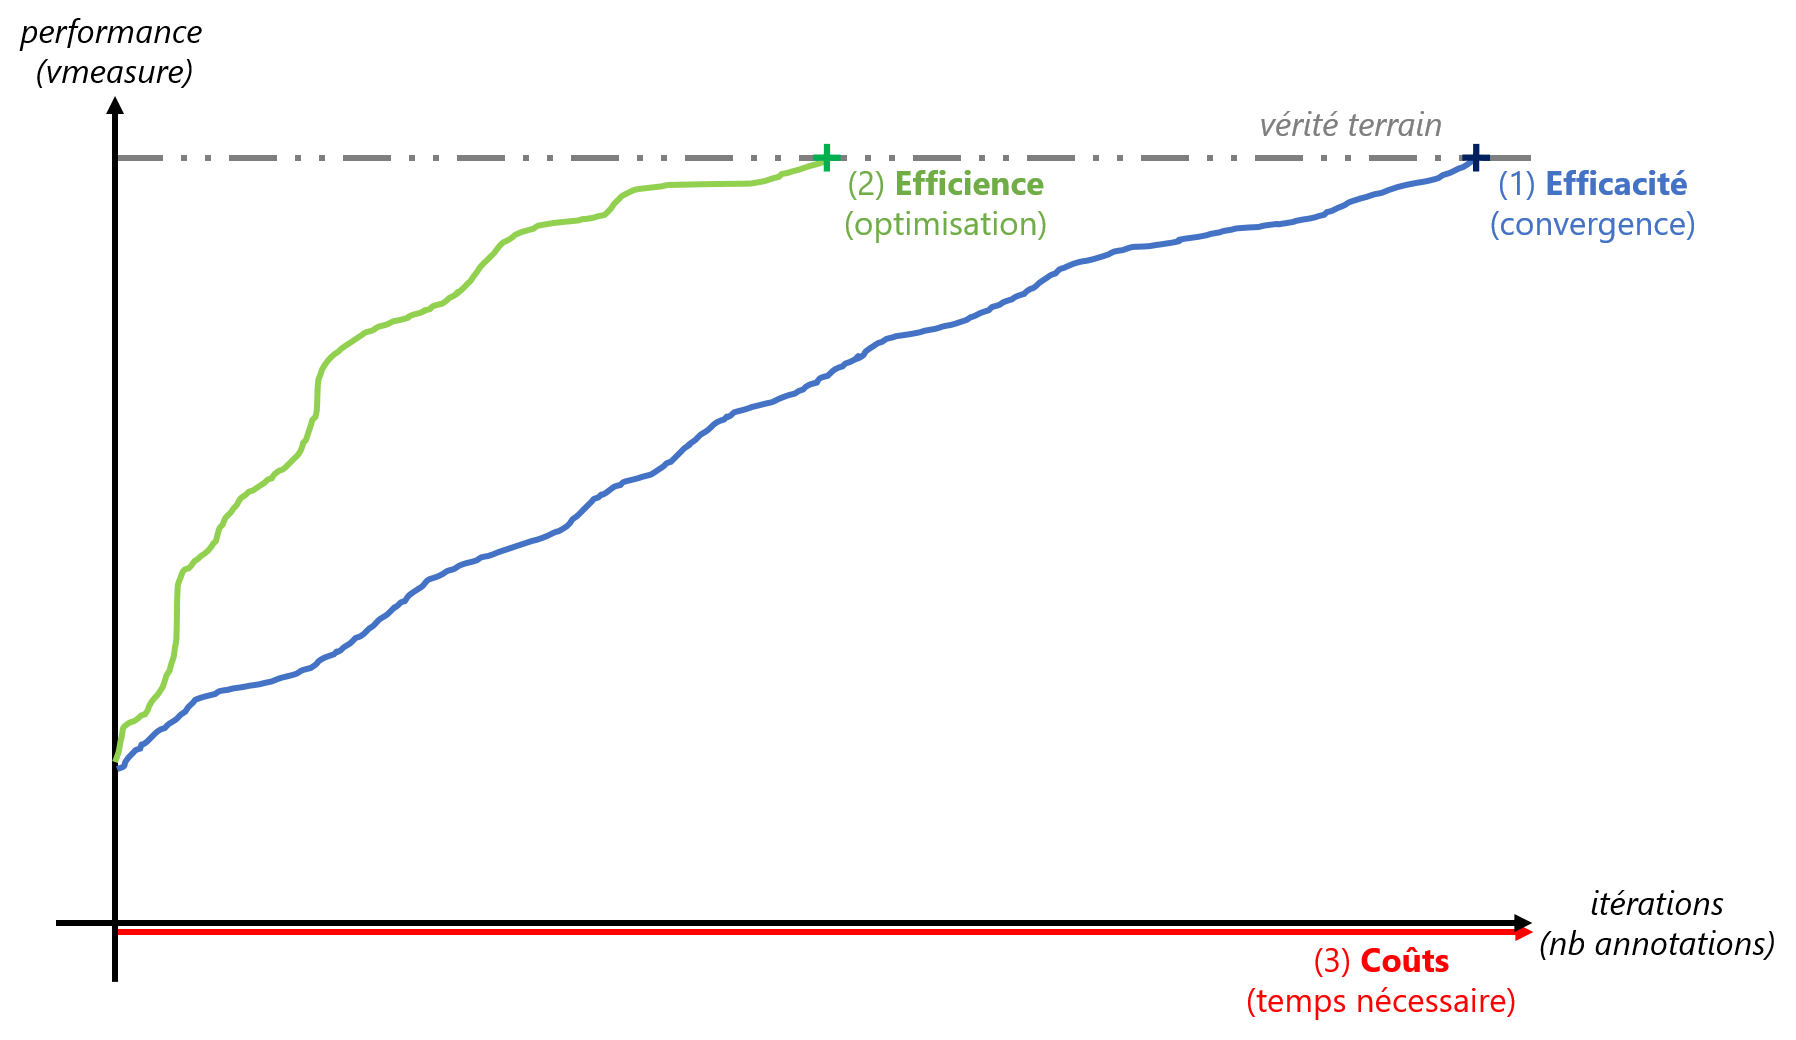
\includegraphics[width=0.8\textwidth]{figures/hypotheses-03-couts}
			\caption{Illustration des études réalisées sur le \textit{clustering} interactif (\textit{étape 3/6}) en schématisant l'évolution de la performance (\textit{accord avec la vérité terrain calculé en v-measure}) d'une base d'apprentissage en cours de construction en fonction du nombre d'itérations de la méthode (\textit{nombre d'annotations par un expert métier}).}
			\label{figure:4.3-HYPOTHESE-COUTS}
		\end{figure}

	\end{tcolorbox}
	
	
	%%%
	%%% Subsection 4.3.1: Étude du temps d'annotation par un expert métier
	%%%
	\subsection{Étude du temps d'annotation par un expert métier}
	\label{section:4.3.1-ETUDE-COUTS-TEMPS-ANNOTATION}
	
		%%% Protocole expérimental.
		\subsubsection{Protocole expérimental}
		
			% Objectif de l'expérience.
			Nous voulons estimer le temps nécessaire à un opérateur pour annoter un lot de contraintes.
			Pour cela, nous allons chronométrer plusieurs expert métiers en train d'annoter un même échantillon et modéliser le nombre de contraintes par minute ainsi que son évolution au cours de plusieurs sessions d'annotation.
			
			% Axiome.
			\begin{leftBarWarning}
				Dans cette étude, nous supposons que les annotateurs de l'expérience connaissent parfaitement le domaine traité dans le jeu de données, et qu'ils sont capables de caractériser sans ambiguïté la similitude entre deux données issues de cet ensemble.
				Afin de pourvoir faire cette hypothèse forte, et ainsi limiter les bruits dans l'analyse des résultats, le jeu de données devra traiter d'un sujet de culture générale (ne nécessitant donc pas de connaissance particulière) et des réviseurs devront supprimer en amont et d'un commun accord les données trop spécifiques.
			\end{leftBarWarning}
			
			% Pseudo-code.
			Pour résumer le protocole expérimental que nous décrivons c-dessous, vous pouvez vous référer au pseudo-code décrit dans Alg.~\ref{algorithm:4.3.1-ETUDE-COUTS-TEMPS-ANNOTATION-PROTOCOLE}.
			%
			\begin{algorithm}[!htb]
				\begin{algorithmic}[1]
					\Require jeu de données annoté (vérité terrain)
					\Require plusieurs réviseurs, plusieurs annotateurs
					\State \textbf{initialisation} définir et revoir le jeu de données entre réviseurs
					\State \textbf{échantillonnage} sélectionner une base de contraintes avec \texttt{samp.rand.full}
					\ForAll{annotateur}
						\While{la base de contraintes n'a pas été entièrement annotée}
							\State \textbf{chronomètre: START}
							\State \textbf{annotation}: annoter une partie des contraintes
							\State \textbf{revue}: revue des contraintes en conflits d'annotation
							\State \textbf{chronomètre: STOP}
							\State \textbf{mesure}: estimer la différence de chronomètre pour cette session
						\EndWhile
					\EndFor
					\State \textbf{modélisation}: entraîner un modèle linéaire généralisé du temps d'annotation
					\State \textbf{simulation}: écrire l'équation du temps d'annotation d'un lot de contraintes
					\Ensure modélisation du temps d'annotation d'un lot de contraintes
				\end{algorithmic}
				\caption{Description en pseudo-code du protocole expérimental de l'étude du temps d'annotation d'un lot de contraintes par un expert métier.}
				\label{algorithm:4.3.1-ETUDE-COUTS-TEMPS-ANNOTATION-PROTOCOLE}
			\end{algorithm}
			
			% Détails de l'expérience : préparation du jeu de données.
			Pour cette étude, nous procéderons en plusieurs étapes.
			D'abord, il faut choisir un jeu de données approprié : pour valider notre hypothèse forte sur les compétence de nos annotateurs, nous cherchons un jeu de données traitant d'un sujet de culture général.
			Pour cette expérience, nous avons donc choisi une collecte des titres d'articles de journaux classés par catégorie de publication (\textit{économie}, \textit{sport},...).
			Comme certains titres peuvent porter à confusion (un titre d'article n'étant pas toujours explicite sur son contenu), deux réviseurs sont chargés de choisir les données les plus explicites sur un échantillon d'un millier de données représentatives des $14$ catégories les plus communes.
			L'échantillon résultant est décrit en annexe~\todo{TODO: ANNEXE JEU DE DONNEES}.
			
			% Détails de l'expérience : sélection des contraintes à annoter. 
			A partir de ces données, nous sélectionnons un lot de $1~000$ contraintes à annoter. Comme nous nous intéressons exclusivement au temps d'annotation pour cette expérience (et que nous ne regardons pas la vitesse de convergence vers la vérité terrain), nous utilisons l'échantillonnage purement aléatoire (\texttt{samp.rand.full}).			
			
			% Détails de l'expérience : annotations et consignes.
			Ensuite ...
			\todo[inline]{A REDIGER: consignes annotateurs}
			\todo[inline]{A REDIGER: description interface}
			
			
			% Détails de l'expérience : modélisation.
			Une fois les sessions d'annotations terminées, nous entraînons un modèle linéaire généralisé (\textit{GLM}) pour estimer le temps d'annotation moyen pour un lot de contraintes. Ce modèle sera caractérisé par le coefficient de détermination généralisé \texttt{R²} de \textit{Cox et Snel}, la log-vraisemblance \texttt{llf} et la log-vraisemblance \texttt{llf\_null} du modèle \textit{null}.
			Nous discuterons aussi de l'évolution de la vitesse d'un opérateur au cours des différentes sessions d'annotation.

			% Référence scripts.
			\begin{leftBarInformation}
				Ces analyses sont réalisées en Python à l'aide des librairies \texttt{datetime} et \texttt{statsmodels} (\cite{seabold:2010}).
				Le projet à importer dans l'outil d'annotation ainsi que les scripts de l'expérience (\textit{notebooks} Python) sont disponibles dans un dossier dédié de~\cite{schild:cognitivefactory-interactive-clustering-comparative-study:2021}.
			\end{leftBarInformation}
			\todo{citation}

		%%% Résultats
		\subsubsection{Résultats obtenus}
		
			% Modélisation du temps d'annotation.
			\todo[inline]{A REDIGER: Description statistiques des résultats}
			\todo[inline]{A REDIGER: Modélisation du temps}
			\todo[inline]{A REDIGER: équation du temps}
			
		
			% Affichage du temps d'annotation.
			La figure~\ref{figure:4.3.1-ETUDE-COUTS-TEMPS-ANNOTATION-SIMULATION} représente cette modélisation du temps d'annotation en comparaison avec les mesures réalisées lors de l'expérience.
			\begin{figure}[!htb]
				\centering
				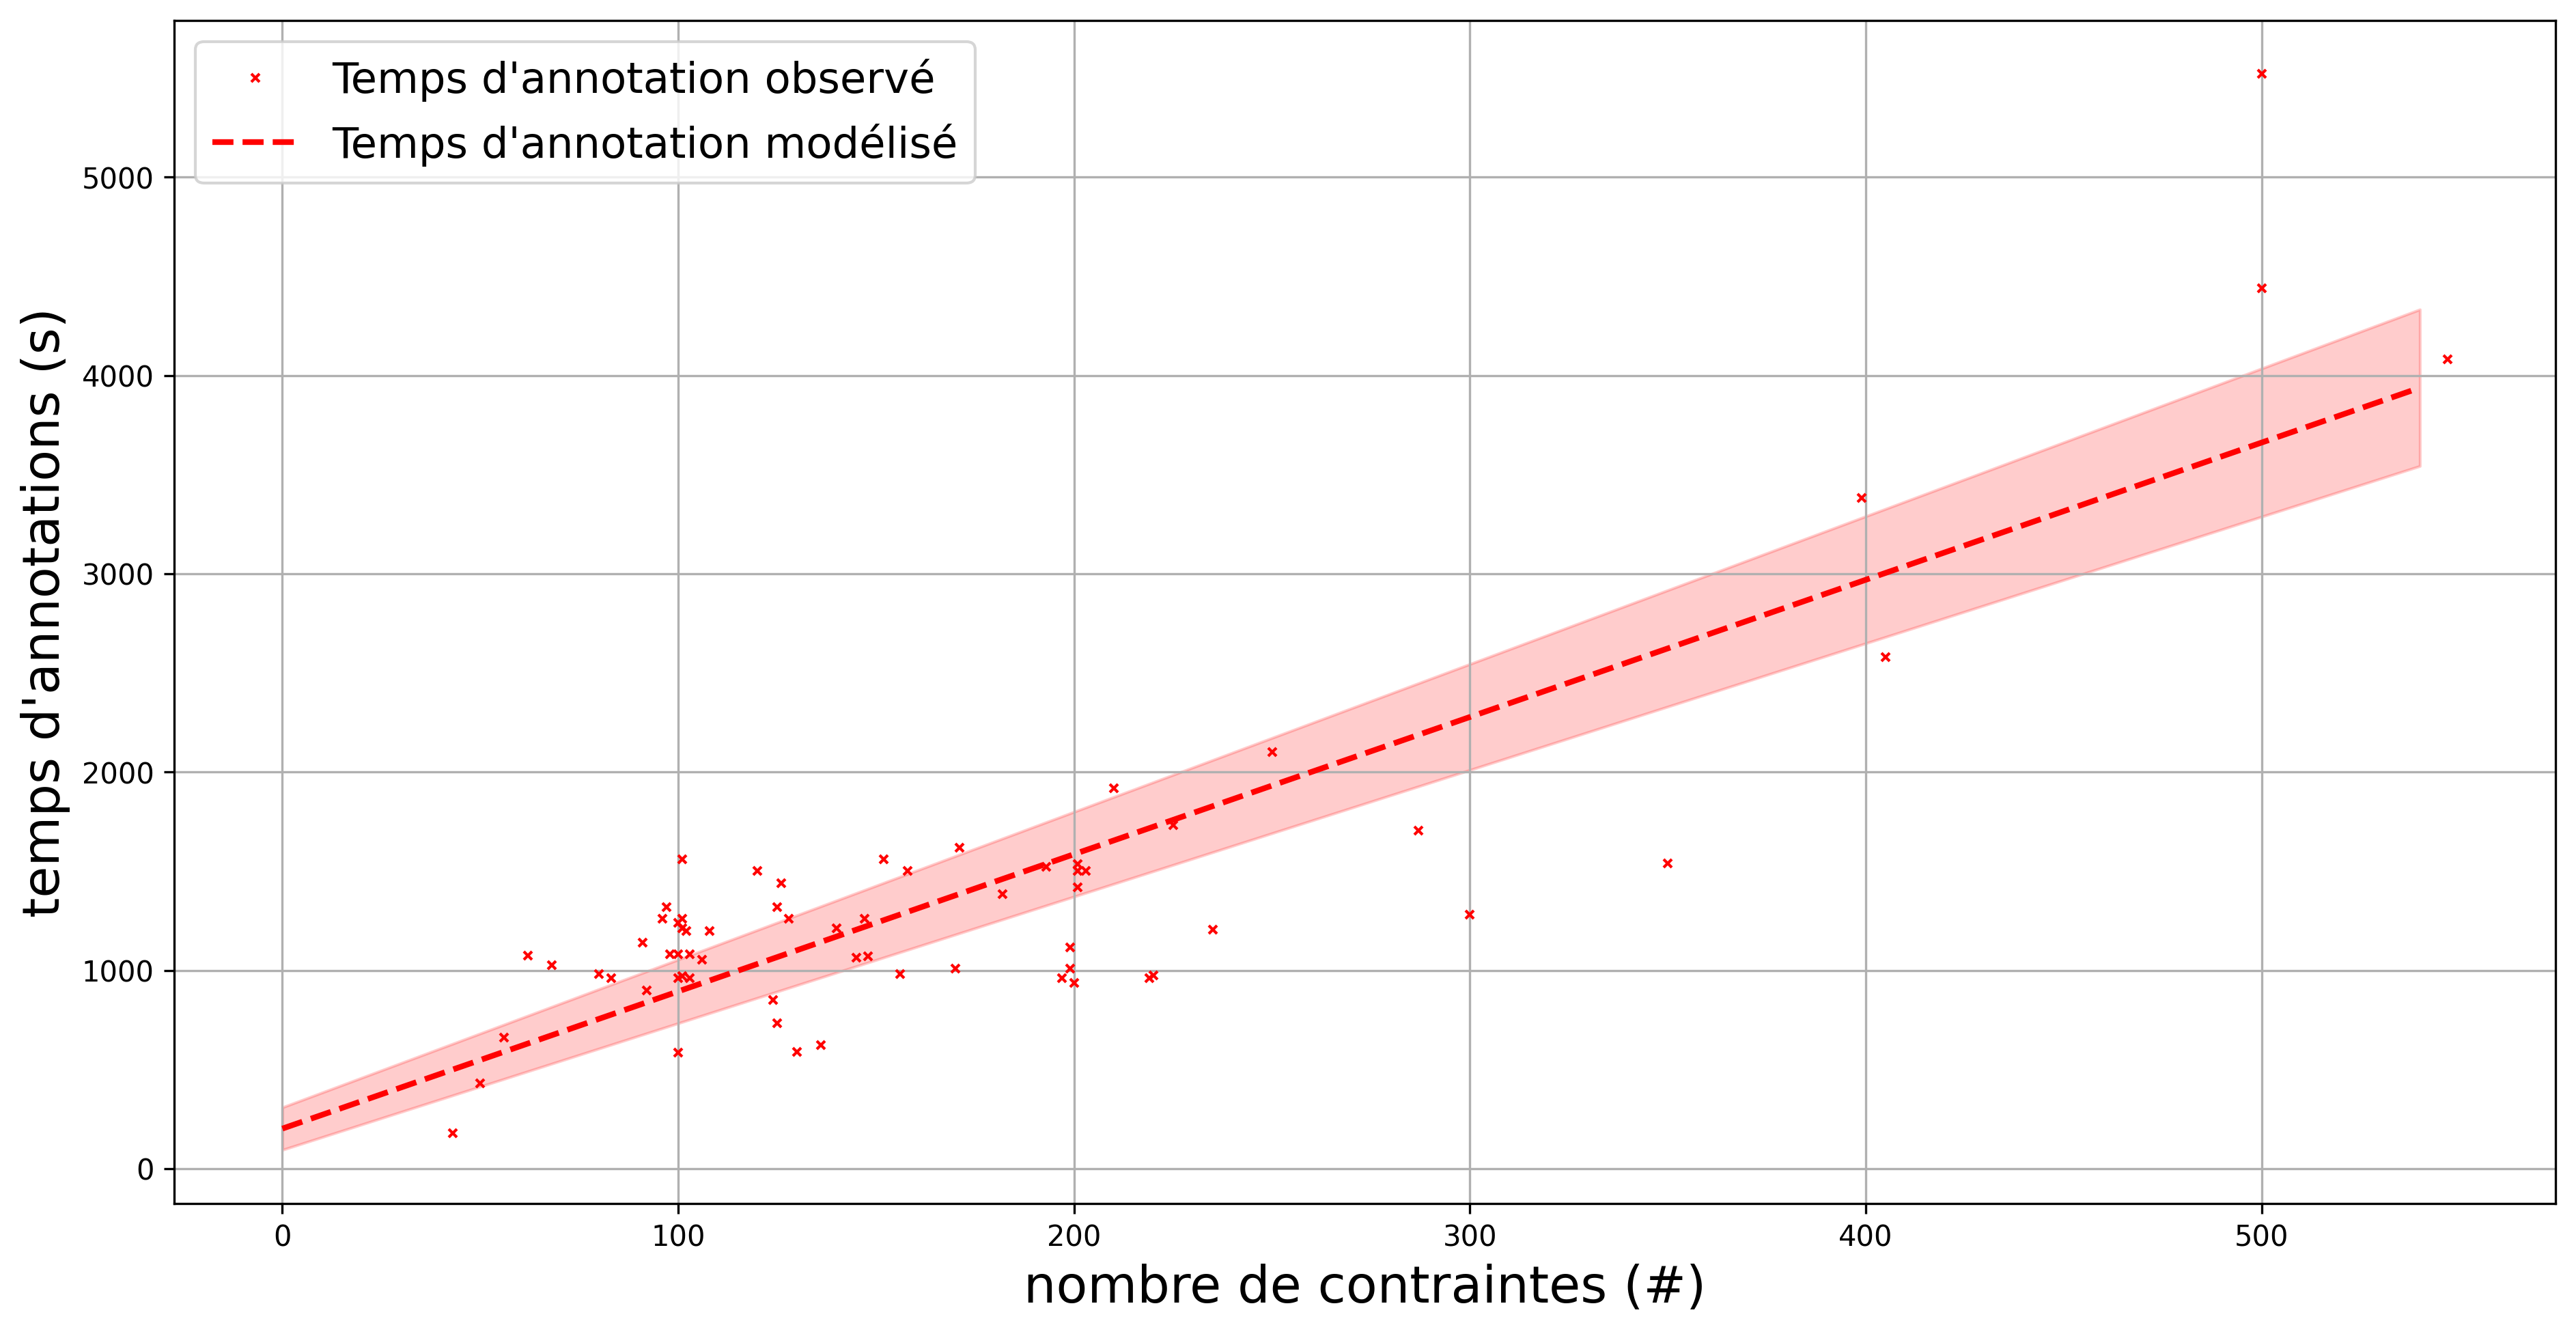
\includegraphics[width=\textwidth]{figures/etude-temps-annotation-1-modelisation-temps}
				\caption{Estimation du temps nécessaire (en secondes) pour annoter un lot de contraintes.}
				\label{figure:4.3.1-ETUDE-COUTS-TEMPS-ANNOTATION-SIMULATION}
			\end{figure}
		
			% Etude de cas.
			La figure~\ref{figure:4.3.1-ETUDE-COUTS-TEMPS-ANNOTATION-EXEMPLE} représente l'évolution de la vitesse d'annotation de quatre opérateurs (les deux plus rapides et les deux plus lents). Ces données sont l'objet d'une étude de cas dans la discussion ci-dessous.
			\begin{figure}[!htb]
				\centering
				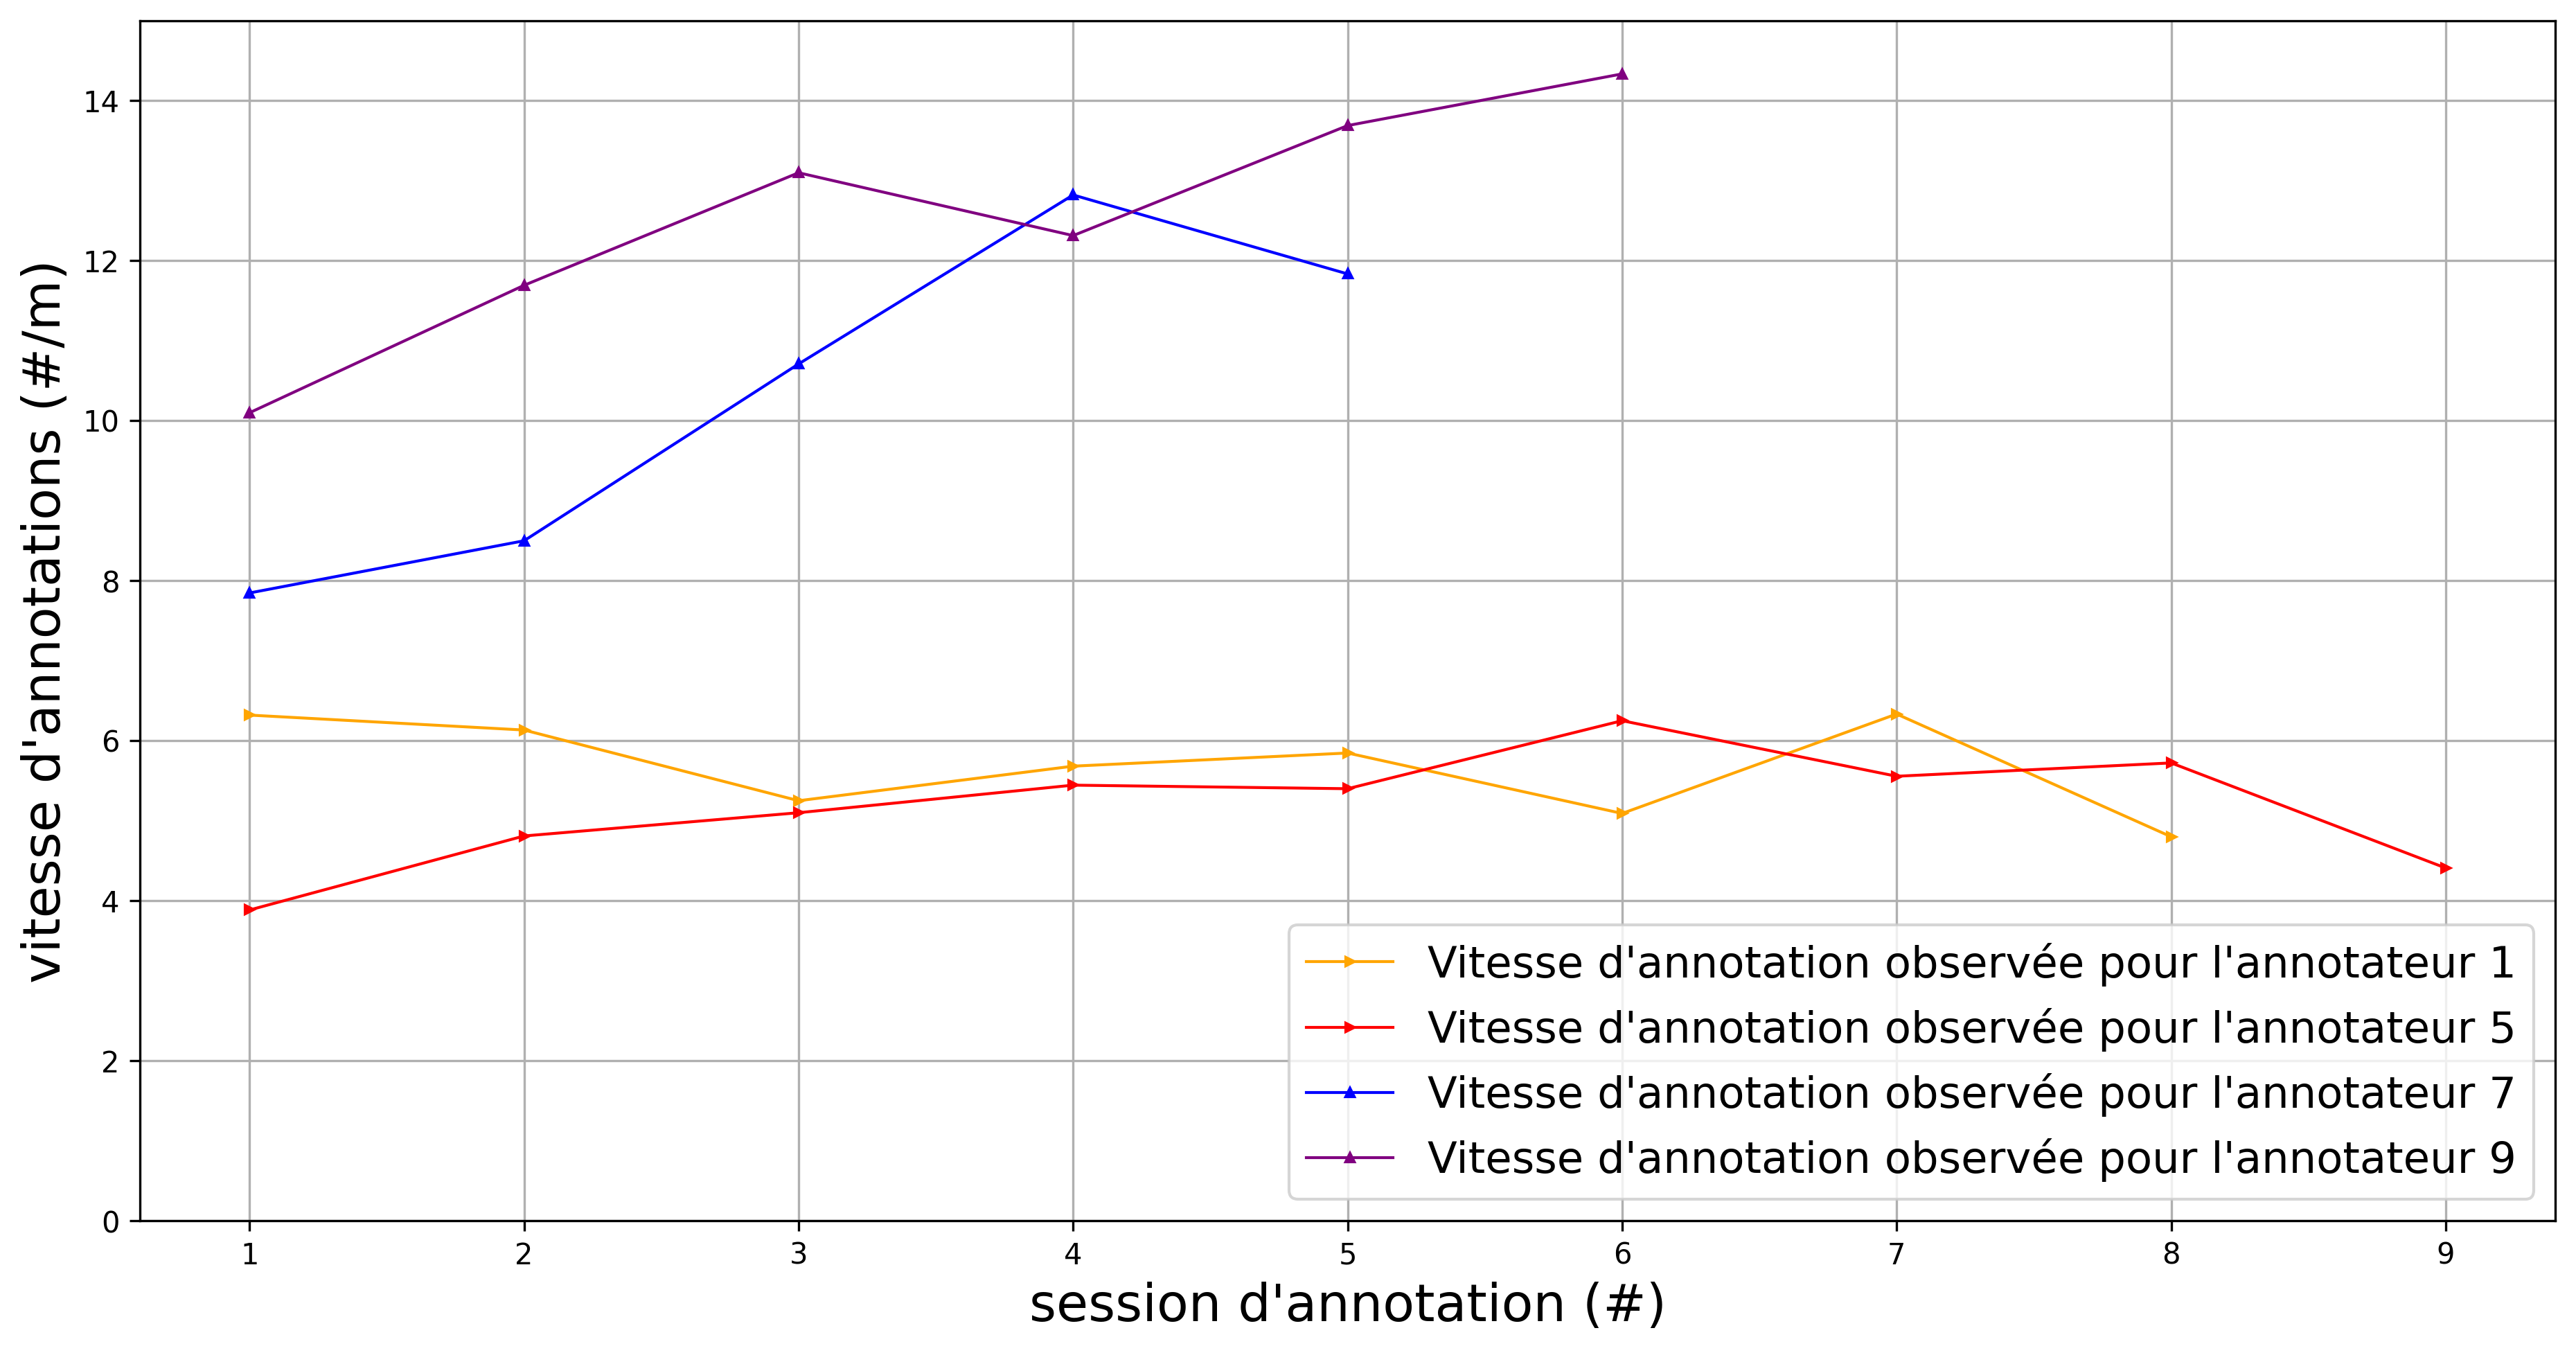
\includegraphics[width=\textwidth]{figures/etude-temps-annotation-3-etude-de-cas}
				\caption{Etude de cas d'évolution de la vitesse d'annotation de contraintes (en contraintes par minutes) en fonction des différentes sessions d'annotations}
				\label{figure:4.3.1-ETUDE-COUTS-TEMPS-ANNOTATION-EXEMPLE}
			\end{figure}

		%%% Discussion
		\subsubsection{Discussion}
		
			\todo[inline]{A REDIGER: Discussion temps moyen}
			\todo[inline]{A REDIGER: Discussion vitesse d'annotation}
	

	%%%
	%%% Subsection 4.3.2: Étude du temps de calcul des algorithmes
	%%%
	\subsection{Étude du temps de calcul des algorithmes}
	\label{section:4.3.2-ETUDE-COUTS-TEMPS-CALCUL}
	
		%%% Protocole expérimental.
		\subsubsection{Protocole expérimental : estimer le temps de calcul des algorithmes du \textit{clustering} interactif}
		
			% Objectif de l'expérience.
			Pour confirmer le choix du paramétrage pour une convergence optimale (cf. hypothèse d'efficience en section~\ref{section:4.2-HYPOTHESE-EFFICIENCE}), nous voulons étudier le temps de calcul de chaque algorithme intervenant dans notre implémentation du \textit{clustering} interactif.
			Pour cela, nous allons chronométrer plusieurs exécutions de ces algorithmes avec différents arguments d'entrée (la taille du jeu de données, le nombre de clusters et le nombre de contraintes annotées, ...) et modéliser le temps de calcul résultant en fonction de ces paramètres.
			
			% Remarques.
			\begin{leftBarWarning}
				Pour utiliser des jeux de données de tailles différentes tout en maîtrisant leur contenu, nous avons dupliqués aléatoirement des données en générant des fautes de frappes. Pour cette étude, nous faisons l'hypothèse que cela n'a pas d'impact majeur sur le temps d'exécution des différents algorithmes.
			\end{leftBarWarning}
			
			% Pseudo-code.
			Pour résumer le protocole expérimental que nous décrivons ci-dessous, vous pouvez vous référer aux pseudo-code décrit dans Alg.~\ref{algorithm:4.3.2-ETUDE-COUTS-TEMPS-CALCUL-PROTOCOLE}.
			%
			\begin{algorithm}[!htb]
				\begin{algorithmic}[1]
					\Require jeu de données annoté (vérité terrain)
					\ForAll{arrangement d'algorithmes et de paramètres à tester}
						\State \textbf{initialisation}: récupérer ou générer le jeu de données
						\If{estimation de la tâche de \textbf{prétraitement}}
							\State \textbf{chronomètre: START}
							\State \textbf{prétraitement (à étudier)}: supprimer le bruit dans les données
							\State \textbf{chronomètre: STOP}
						\ElsIf {estimation de la tâche de \textbf{vectorisation}}
							\State \textbf{prétraitement}: supprimer le bruit dans les données avec \texttt{prep.simple}
							\State \textbf{chronomètre: START}
							\State \textbf{vectorisation (à étudier)}: transformer les données en vecteurs
							\State \textbf{chronomètre: STOP}
						\ElsIf {estimation de la tâche de \textbf{clustering}}
							\State \textbf{prétraitement}: supprimer le bruit dans les données avec \texttt{prep.simple}
							\State \textbf{vectorisation}: transformer les données en vecteurs avec \texttt{vect.tfidf}
							\State \textbf{échantillonnage initial}: sélectionner une base de contraintes avec \texttt{samp.rand.full}
							\State \textbf{simulation d'annotation}: ajouter des contraintes en utilisant la vérité terrain
							\State \textbf{chronomètre: START}
							\State \textbf{clustering (à étudier)}: regrouper les données par similarité
							\State \textbf{chronomètre: STOP}
						\ElsIf {estimation de la tâche d'\textbf{échantillonnage}}
							\State \textbf{prétraitement}: supprimer le bruit dans les données avec \texttt{prep.simple}
							\State \textbf{vectorisation}: transformer les données en vecteurs avec \texttt{vect.tfidf}
							\State \textbf{échantillonnage initial}: sélectionner une base de contraintes avec \texttt{samp.rand.full}
							\State \textbf{simulation d'annotation}: ajouter des contraintes en utilisant la vérité terrain
							\State \textbf{clustering initial}: regrouper les données par similarité avec \texttt{clust.kmeans.cop}
							\State \textbf{chronomètre: START}
							\State \textbf{échantillonnage (à étudier)}: sélectionner de nouvelles contraintes à annoter
							\State \textbf{chronomètre: STOP}
						\EndIf
						\State \textbf{mesure}: estimer la différence de chronomètre pour cet algorithme
					\EndFor
					\ForAll{algorithme à modéliser}
						\State \textbf{cadrage}: définir les facteurs et les interactions intervenant dans la modélisation
						\State \textbf{simplification}: restreindre la modélisation aux facteurs les plus corrélés
						\State \textbf{modélisation}: entraîner un modèle linéaire généralisé avec les facteurs retenus
						\State \textbf{simulation}: écrire l'équation du temps d'exécution avec des paramètres obtenus
					\EndFor
					\Ensure modélisation du temps d'exécution des différents algorithmes
				\end{algorithmic}
				\caption{Description en pseudo-code du protocole expérimental de l'étude du temps d'exécution des algorithmes du \textit{clustering} interactif}
				\label{algorithm:4.3.2-ETUDE-COUTS-TEMPS-CALCUL-PROTOCOLE}
			\end{algorithm}
			
			% Description des tâches, des algorithmes et des contextes.
			Pour cette étude, nous lançons plusieurs exécutions de chaque algorithme de notre implémentation du \textit{clustering} interactif (cf. section~\ref{section:3.3-DESCRIPTION-IMPLEMENTATION}) avec différentes variations de contexte d'utilisation. Cela comprend les tâches, algorithmes et contextes d'utilisation suivants :
			%
			\begin{enumerate}
				% Prétraitement.
				\item le \textbf{prétraitement} des données...
					\begin{itemize}
						\item avec les algorithmes suivants : \textbf{simple} (noté \texttt{prep.simple}), \textbf{avec lemmatisation} (noté \texttt{prep.lemma}) et \textbf{avec filtres} (noté \texttt{prep.filter}) ;
						\item avec les contextes d'utilisation suivants : \textbf{nombre de données} (variant de $1~000$ à $5~000$ par pas de $1~000$, noté $\texttt{dataset\_size}$) ;
					\end{itemize}
				% Vectorisation.
				\item la \textbf{vectorisation} des données...
					\begin{itemize}
						\item avec les algorithmes suivants : \textbf{TF-IDF} (noté \texttt{vect.tfidf}) et \textbf{SpaCy} (noté \texttt{vect.frcorenewsmd}) ;
						\item avec les contextes d'utilisation suivants : \textbf{nombre de données} (variant de $1~000$ à $5~000$ par pas de $1~000$, noté $\texttt{dataset\_size}$) ;
						\item précédé par un prétraitement \textbf{simple} ;
					\end{itemize}
				% Clustering.
				\item le \textbf{\textit{clustering} sous contraintes} des données...
					\begin{itemize}
						\item avec les algorithmes suivants : \textbf{KMeans} (modèle \textit{COP} noté \texttt{clust.kmeans.cop}), \textbf{Hiérarchique} (lien \textit{single} noté \texttt{clust.hier.sing} ; lien \textit{complete} noté \texttt{clust.hier.comp} ; lien \textit{average} noté \texttt{clust.hier.avg} ; lien \textit{ward} noté \texttt{clust.hier.ward}) et \textbf{Spectral} (modèle \textit{SPEC} noté \texttt{clust.spec}) ;
						\item avec les contextes d'utilisation suivants : \textbf{nombre de données} (variant de $1~000$ à $5~000$ par pas de $1~000$, noté $\texttt{dataset\_size}$), le \textbf{nombre de contraintes annotés} (variant de $0$ à $5~000$ par pas de $500$, noté $\texttt{previous\_nb\_constraints}$) et le \textbf{nombre de \textit{clusters} à trouver} (variant de $5$ à $50$ par pas de $5$, noté $\texttt{algorithm\_nb\_clusters}$) ;
						\item précédé par un prétraitement \textbf{simple} et une vectorisation \textbf{TF-IDF} et un échantillonnage initial \textbf{purement aléatoire} ;
					\end{itemize}
				% Sampling.
				\item l'\textbf{échantillonnage} des contraintes à annoter...
					\begin{itemize}
						\item avec les algorithmes suivants : \textbf{purement aléatoire} (noté \texttt{samp.random.full}), \textbf{pseudo-aléatoire} (noté \texttt{samp.random.same}), \textbf{même cluster et étant les plus éloignées} (noté \texttt{samp.farhtest.same}) et \textbf{clusters différents et étant les plus proches} (noté \texttt{samp.closest.diff}) ;
						\item avec les contextes d'utilisation suivants : \textbf{nombre de données} (variant de $1~000$ à $5~000$ par pas de $1~000$, noté $\texttt{dataset\_size}$), le \textbf{nombre de contraintes annotés} (variant de $0$ à $5~000$ par pas de $500$, noté $\texttt{previous\_nb\_constraints}$), le \textbf{nombre de \textit{clusters} existant} (variant de $10$ à $50$ par pas de $10$, noté $\texttt{previous\_nb\_clusters}$) et le \textbf{nombre de contraintes à sélectionner} (variant de $50$ à $250$ par pas de $50$, noté $\texttt{algorithm\_nb\_constraints}$) ;
						\item précédé par un prétraitement \textbf{simple}, une vectorisation \textbf{TF-IDF}, un \textit{clustering} initial \textbf{KMeans} (modèle \textit{COP}) et un échantillonnage initial \textbf{purement aléatoire} ;
					\end{itemize}
			\end{enumerate}
			
			Il y a donc $8~825$ combinaisons d'algorithmes (\texttt{15} pour le prétraitement, $10$ pour la vectorisation, $3~330$ pour le \textit{clustering}, $5~550$ pour l'échantillonnage), et chaque combinaison est répétée $5$ fois pour contrer les aléas statistiques des exécutions.
			De plus, chaque jeu de données est généré $5$ fois pour contrer les aléas statistiques de création, donc il y a $220~625$ exécutions d'algorithmes ($375$ pour le prétraitement, $250$ pour la vectorisation, $82~500$ pour le \textit{clustering}, $137~500$ pour l'échantillonnage).
			
			% Description de la modélisation.
			Sur la base de ces mesures, nous cherchons à modéliser le temps d'exécution de chaque algorithme en fonction de son contexte d'utilisation (dépendant de ses arguments d'entrée\footnote{Les arguments d'entrée peuvent influencer le contexte d'utilisation à partir du du : nombre de données, nombre de contraintes annotées, nombre de contraintes à sélectionner, nombre de \textit{clusters} existant, nombre de \textit{clusters} à trouver}), et les interactions doubles entre paramètres sont envisagées.
			Afin de réduire la complexité des modélisations, nous ordonnons les interactions de facteurs possibles en fonction de leur corrélation avec le temps mesuré (la corrélation \texttt{r} de \textit{Pearson} est utilisée) et nous nous limitons aux variables responsables d'un maximum de la variance des mesures (la méthode d'\textit{Elbow} est utilisée pour choisir les facteurs pertinents).
			Sur cette base, nous entraînons un modèle linéaire généralisé (\textit{GLM}) pour représenter le temps d'exécution moyen de l'algorithme : ce modèle sera caractérisé par le coefficient de détermination généralisé \texttt{R²} de \textit{Cox et Snel}, la log-vraisemblance \texttt{llf} et la log-vraisemblance \texttt{llf\_null} du modèle \textit{null}.
			Pour finir, nous discuterons des valeurs des coefficients obtenus sur l'impact du temps d'exécution.
			
			% Référence scripts.
			\begin{leftBarInformation}
				Ces analyses sont réalisées en Python à l'aide des librairies \texttt{datetime} et \texttt{statsmodels} (\cite{seabold:2010}).
				Les scripts de l'expérience (\textit{notebooks} Python) sont disponibles dans un dossier dédié de~\cite{schild:cognitivefactory-interactive-clustering-comparative-study:2021}.
			\end{leftBarInformation}
			\todo{citation}

		%%% Résultats
		\subsubsection{Résultats obtenus}
				
			%%% Prétraitements
			
			% Première analyse.
			En ce qui concerne la tâche de \textbf{prétraitement}, une première analyse montre que les modélisations des trois implémentations sont similaires (\texttt{p-valeur}: $> 0.980$). Nous ferons donc une seule modélisation.
			
			% Modélisation du temps de calcul (prep.simple + prep.lemma + prep.filter).
			Pour les algorithmes de prétraitements (\texttt{prep.simple}, \texttt{prep.lemma} et \texttt{prep.filter}), l'analyse de la corrélation des facteurs avec les mesures de temps d'exécution indique qu'une modélisation minimale et suffisante peut être réalisée à partir du facteur $\texttt{dataset\_size}$ (\texttt{r}: $0.997$).
			Le modèle linéaire généralisé retenu (\texttt{R²}: $> 0.999$, \texttt{llf}: $-379.35$, \texttt{llf\_null}: $-1~353.98$) nous permet de déduire l'équation suivante\footnote{Cette déduction est en accord avec la complexité théorique de l'algorithme qui est en $ \mathcal{O}(\texttt{dataset\_size}) $.}\todo{ref annexe} :
			%
			\begin{equation}
				time(prep)
				\simeq 8.39 \cdot 10^{-1} + 6.31 \cdot 10^{-3} \cdot \texttt{dataset\_size}
			\end{equation}
			
			% Affichage du temps de calcul.
			La figure~\ref{figure:4.3.2-ETUDE-COUTS-TEMPS-CALCUL-MODELISATION-PREPROCESSING} représente cette modélisation du temps de calcul des algorithmes de prétraitements en comparaison avec les mesures réalisées lors de l'expérience.
			\newline
			%		
			\begin{figure}[!htb]
				\centering
				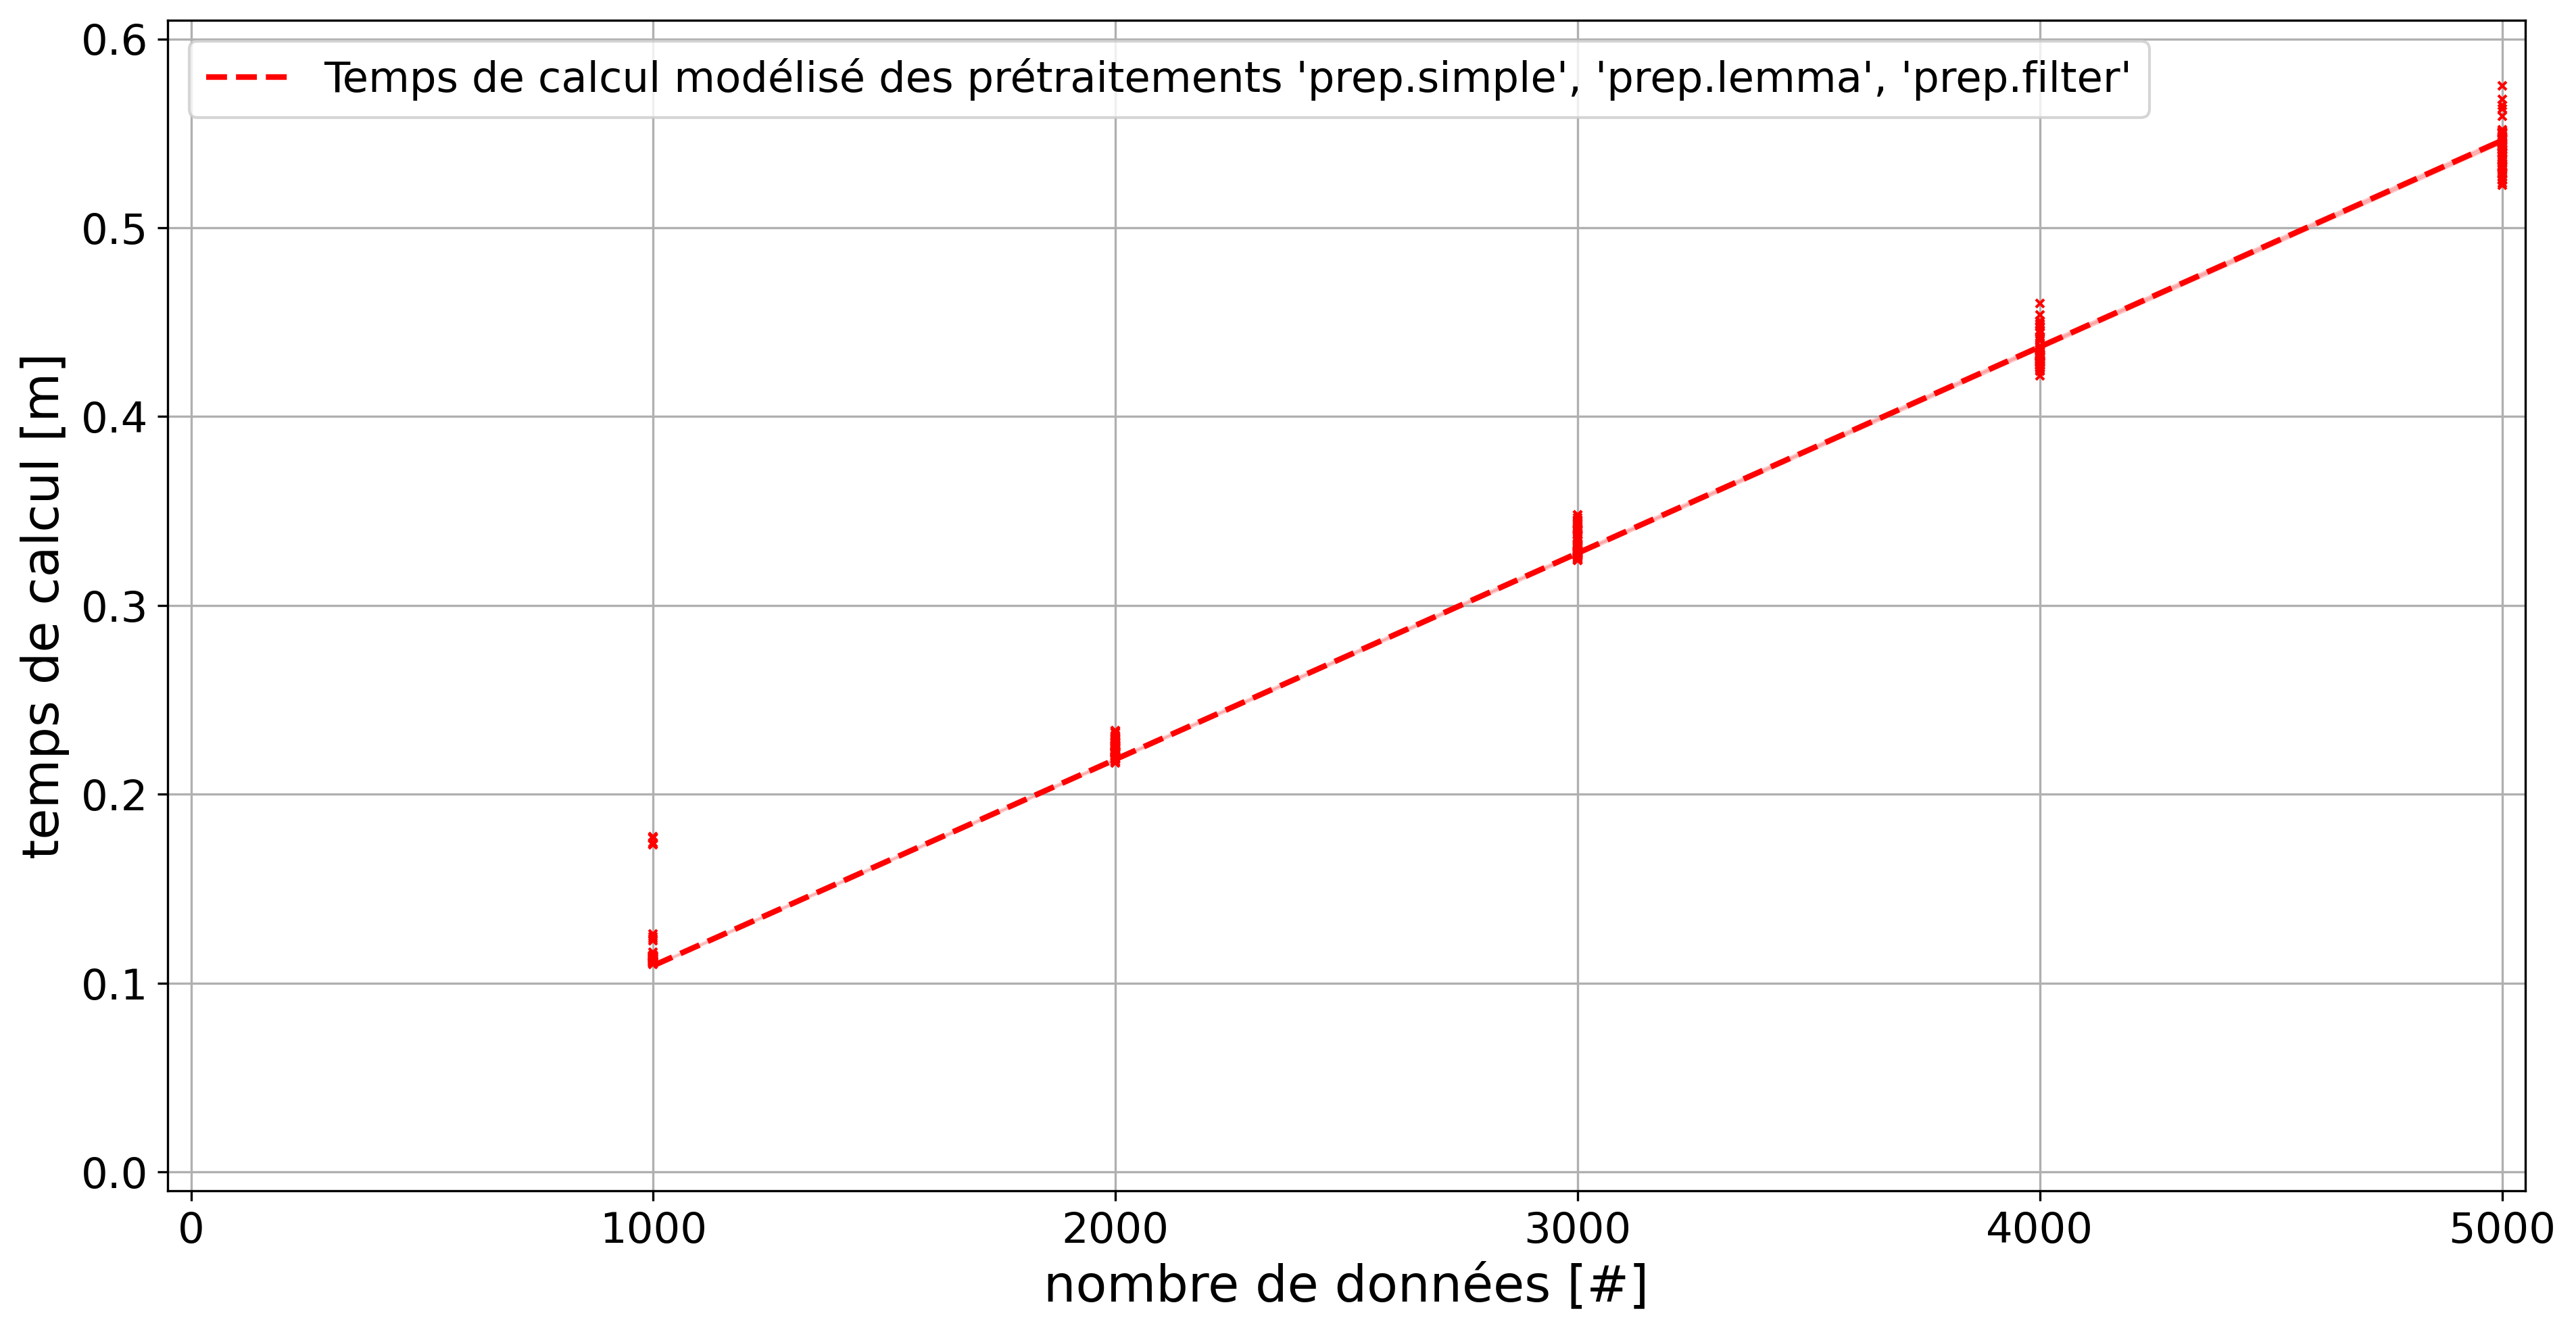
\includegraphics[width=0.8\textwidth]{figures/etude-temps-calcul-modelisation-1prep}
				\caption{Estimation du temps nécessaire (en secondes) pour effectuer une tâche de \textbf{prétraitement} en fonction du nombre de données à traiter. Les paramétrages \texttt{prep.simple}, \texttt{prep.lemma} et \texttt{prep.filter} ayant des temps de calculs similaires, leurs modélisations n'ont pas été séparées.}
				\label{figure:4.3.2-ETUDE-COUTS-TEMPS-CALCUL-MODELISATION-PREPROCESSING}
			\end{figure}
			
			%%% Vectorization
			
			% Première analyse.
			En ce qui concerne la tâche de \textbf{vectorisation}, une première analyse montre que les modélisations des deux implémentations sont différentiables  (\texttt{p-valeur}: $< 10^{-3}$). Nous ferons donc une modélisation par algorithme.
		
			% Modélisation du temps de calcul (vect.tfidf).
			Pour les algorithmes de vectorisation \texttt{vect.tfidf}, l'analyse de la corrélation des facteurs avec les mesures de temps d'exécution indique qu'une modélisation minimale et suffisante peut être réalisée à partir du facteur $\texttt{dataset\_size}$ (\texttt{r}: $0.977$).
			Le modèle linéaire généralisé retenu (\texttt{R²}: $> 0.999$, \texttt{llf}: $262.35$, \texttt{llf\_null}: $70.04$) nous permet de déduire l'équation suivante\footnote{Cette déduction est en accord avec la complexité théorique de l'algorithme qui est en $ \mathcal{O}(\texttt{dataset\_size}) $.}\todo{ref annexe} :
			%
			\begin{equation}
				time(vect.tfidf)
				\simeq -1.40 \cdot 10^{-2} + 9.54 \cdot 10^{-5} \cdot \texttt{dataset\_size}
			\end{equation}
			
			% Modélisation du temps de calcul (vect.frcorenewsmd).
			Pour les algorithmes de vectorisation \texttt{vect.frcorenewsmd}, l'analyse de la corrélation des facteurs avec les mesures de temps d'exécution indique qu'une modélisation minimale et suffisante peut être réalisée à partir du facteur $\texttt{dataset\_size}$ (\texttt{r}: $0.983$).
			Le modèle linéaire généralisé retenu (\texttt{R²}: $> 0.999$, \texttt{llf}: $-186.80$, \texttt{llf\_null}: $-399.39$) nous permet de déduire l'équation suivante\footnote{Cette déduction est en accord avec la complexité théorique de l'algorithme qui est en $ \mathcal{O}(\texttt{dataset\_size}) $.}\todo{ref annexe} :
			%
			\begin{equation}
				time(vect.frcorenewsmd)
				\simeq 1.89 + 4.11 \cdot 10^{-3} \cdot \texttt{dataset\_size}
			\end{equation}
			
			% Affichage du temps de calcul.
			La figure~\ref{figure:4.3.2-ETUDE-COUTS-TEMPS-CALCUL-MODELISATION-VECTORIZATION} représente ces modélisations de temps de calcul des algorithmes de vectorisation en comparaison avec les mesures réalisées lors de l'expérience.
			\newline
			%
			\begin{figure}[!htb]
				\centering
				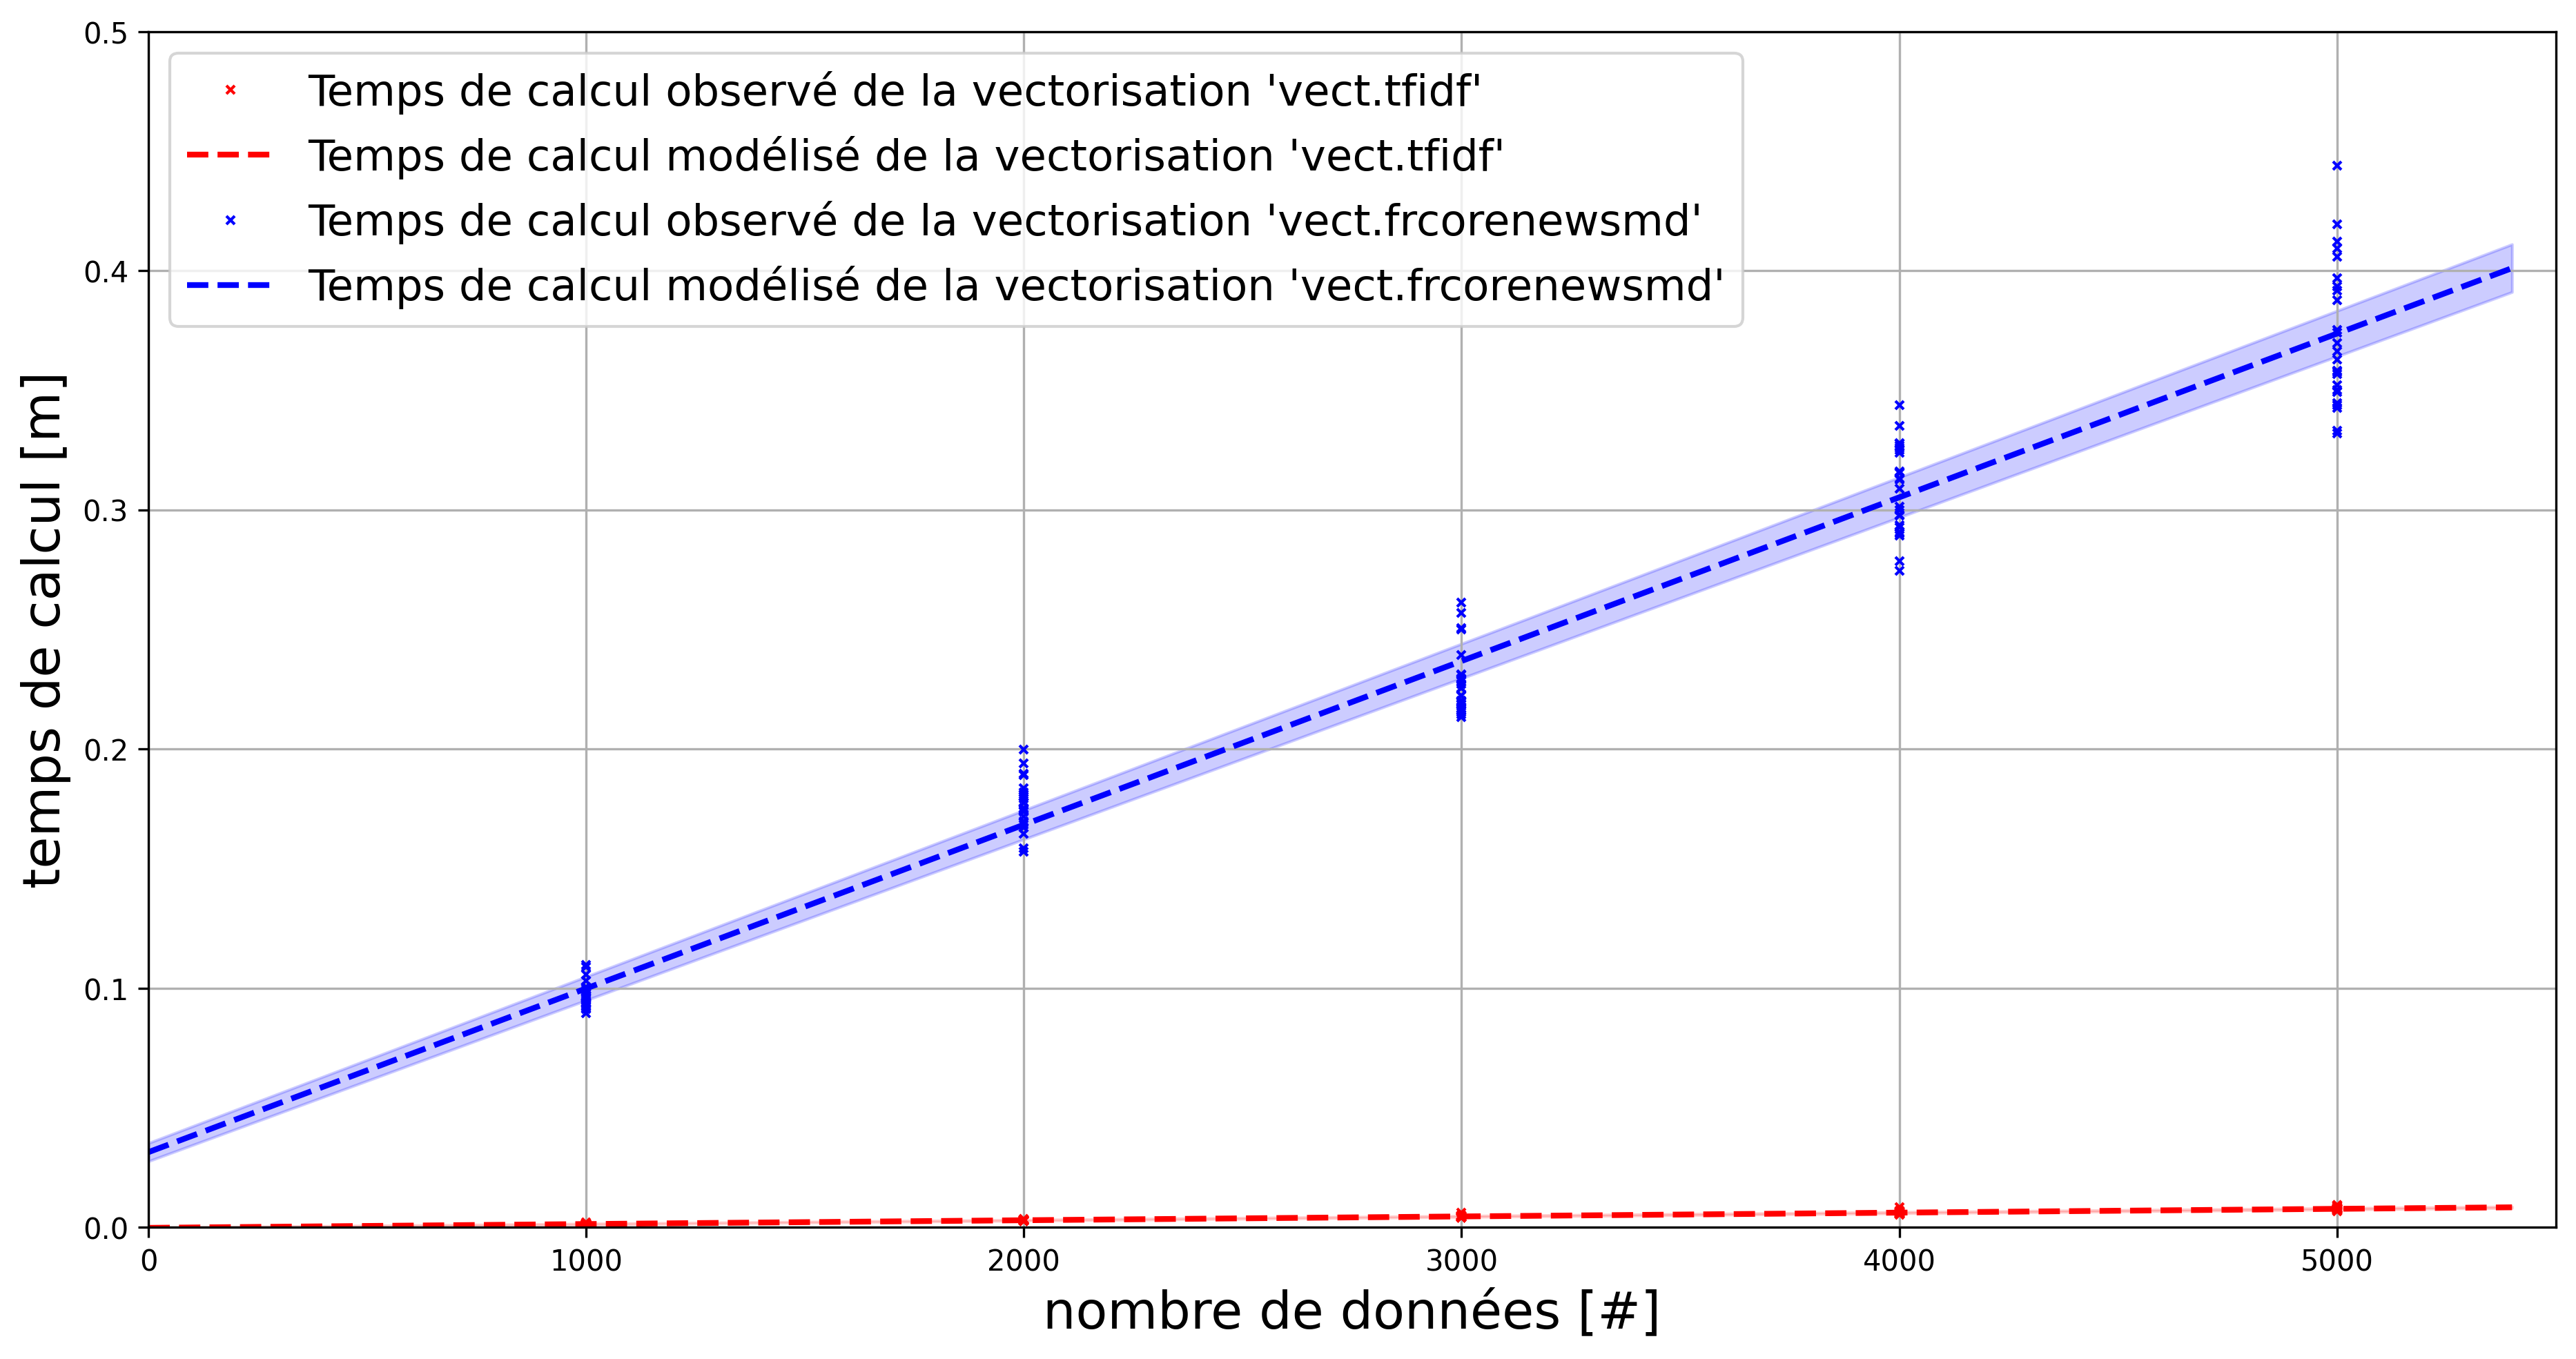
\includegraphics[width=0.8\textwidth]{figures/etude-temps-calcul-modelisation-2vect}
				\caption{Estimation du temps nécessaire (en secondes) pour effectuer une tâche de \textbf{vectorisation} en fonction du nombre de données à traiter.}
				\label{figure:4.3.2-ETUDE-COUTS-TEMPS-CALCUL-MODELISATION-VECTORIZATION}
			\end{figure}
			
			%%% Clustering
			
			% Première analyse.
			En ce qui concerne la tâche de \textbf{\textit{clustering} sous contraintes}, une première analyse montre que les modélisations des six implémentations sont différentiables  (\texttt{p-valeur}: $<$ \texttt{$10^{-3}$}). Nous ferons donc une modélisation par algorithme.
			
			% Modélisation du temps de calcul (clust.kmeans.cop).
			Pour les algorithmes du \textit{clustering} sous contraintes \texttt{clust.kmeans.cop}, l'analyse de la corrélation des facteurs avec les mesures de temps d'exécution indique qu'une modélisation minimale et suffisante peut être réalisée à partir du facteur $\texttt{dataset\_size}$ (\texttt{r}: $0.837$).
			Le second facteur le plus corrélé (mais non retenu) est l'interaction $\texttt{dataset\_size}^{2} \cdot algorithm\_nb\_clusters$ (\texttt{r}: $0.545$).
			Le modèle linéaire généralisé retenu (\texttt{R²}: $0.904$, \texttt{llf}: $-9.20 \cdot 10^{4}$, \texttt{llf\_null}: $-1.00 \cdot 10^{5}$) nous permet de déduire l'équation suivante\todo{ref annexe} :
			%
			\begin{equation}
				time(clust.kmeans.cop)
				\simeq -2.40 \cdot 10^{2} + 2.11 \cdot 10^{-1} \cdot \texttt{dataset\_size}
			\end{equation}
			
			% Modélisation du temps de calcul (clust.hier.sing).
			Pour les algorithmes du \textit{clustering} sous contraintes \texttt{clust.hier.sing}, l'analyse de la corrélation des facteurs avec les mesures de temps d'exécution indique qu'une modélisation minimale et suffisante peut être réalisée à partir du facteur $\texttt{dataset\_size}^{2}$ (\texttt{r}: $0.940$).
			Le second facteur le plus corrélé (mais non retenu) est l'interaction $\texttt{dataset\_size}^{2} \cdot algorithm\_nb\_clusters$ (\texttt{r}: $0.729$).
			Le modèle linéaire généralisé retenu (\texttt{R²}: $> 0.999$, \texttt{llf}: $-5.38 \cdot 10^{4}$, \texttt{llf\_null}: $-6.10 \cdot 10^{4}$) nous permet de déduire l'équation suivante\todo{ref annexe} :
			%
			\begin{equation}
				time(clust.hier.sing)
				\simeq -8.87 \cdot 10^{2} + 6.37 \cdot 10^{-4} \cdot \texttt{dataset\_size}^{2}
			\end{equation}
			
			% Modélisation du temps de calcul (clust.hier.comp).
			Pour les algorithmes du \textit{clustering} sous contraintes \texttt{clust.hier.comp}, l'analyse de la corrélation des facteurs avec les mesures de temps d'exécution indique qu'une modélisation minimale et suffisante peut être réalisée à partir du facteur $\texttt{dataset\_size}^{2}$ (\texttt{r}: $0.938$).
			Le second facteur le plus corrélé (mais non retenu) est l'interaction $\texttt{dataset\_size}^{2} \cdot algorithm\_nb\_clusters$ (\texttt{r}: $0.736$).
			Le modèle linéaire généralisé retenu (\texttt{R²}: $> 0.999$, \texttt{llf}: $-5.40 \cdot 10^{4}$, \texttt{llf\_null}: $-6.11 \cdot 10^{4}$) nous permet de déduire l'équation suivante\todo{ref annexe} :
			%
			\begin{equation}
				time(clust.hier.comp)
				\simeq -9.25 \cdot 10^{2} + 6.42 \cdot 10^{-4} \cdot \texttt{dataset\_size}^{2}
			\end{equation}

			% Modélisation du temps de calcul (clust.hier.avg).
			Pour les algorithmes du \textit{clustering} sous contraintes \texttt{clust.hier.avg}, l'analyse de la corrélation des facteurs avec les mesures de temps d'exécution indique qu'une modélisation minimale et suffisante peut être réalisée à partir du facteur $\texttt{dataset\_size}^{2}$ (\texttt{r}: $0.915$).
			Le second facteur le plus corrélé (mais non retenu) est l'interaction $\texttt{dataset\_size}^{2} \cdot algorithm\_nb\_clusters$ (\texttt{r}: $0.713$).
			Le modèle linéaire généralisé retenu (\texttt{R²}: $0.942$, \texttt{llf}: $-5.82 \cdot 10^{4}$, \texttt{llf\_null}: $-6.45 \cdot 10^{4}$) nous permet de déduire l'équation suivante\todo{ref annexe} :
			%
			\begin{equation}
				time(clust.hier.avg)
				\simeq -1.10 \cdot 10^{3} + 1.02 \cdot 10^{-3} \cdot \texttt{dataset\_size}^{2}
			\end{equation}

			% Modélisation du temps de calcul (clust.hier.ward).
			Pour les algorithmes du \textit{clustering} sous contraintes \texttt{clust.hier.ward}, l'analyse de la corrélation des facteurs avec les mesures de temps d'exécution indique qu'une modélisation minimale et suffisante peut être réalisée à partir du facteur $\texttt{dataset\_size}^{2}$ (\texttt{r}: $0.945$).
			Le second facteur le plus corrélé (mais non retenu) est l'interaction $\texttt{dataset\_size}^{2} \cdot algorithm\_nb\_clusters$ (\texttt{r}: $0.734$).
			Le modèle linéaire généralisé retenu (\texttt{R²}: $> 0.999$, \texttt{llf}: $-5.39 \cdot 10^{4}$, \texttt{llf\_null}: $-6.14 \cdot 10^{4}$) nous permet de déduire l'équation suivante\todo{ref annexe} :
			%
			\begin{equation}
				time(clust.hier.ward)
				\simeq -9.79 \cdot 10^{2} + 6.82 \cdot 10^{-4} \cdot \texttt{dataset\_size}^{2}
			\end{equation}
			
			% Modélisation du temps de calcul (clust.spec).
			Pour les algorithmes du \textit{clustering} sous contraintes \texttt{clust.spec}, l'analyse de la corrélation des facteurs avec les mesures de temps d'exécution indique qu'une modélisation minimale et suffisante peut être réalisée à partir du facteur $\texttt{dataset\_size}^{2}$ (\texttt{r}: $0.658$).
			Le second facteur le plus corrélé (mais non retenu) est l'interaction $\texttt{dataset\_size}^{2} \cdot algorithm\_nb\_clusters$ (\texttt{r}: $0.595$).
			Le modèle linéaire généralisé retenu (\texttt{R²}: $0.534$, \texttt{llf}: $-7.88 \cdot 10^{5}$, \texttt{llf\_null}: $-8.27 \cdot 10^{5}$) nous permet de déduire l'équation suivante\todo{ref annexe} :
			%
			\begin{equation}
				time(clust.spec)
				\simeq 11.00 + 7.56 \cdot 10^{-6} \cdot \texttt{dataset\_size}^{2}
			\end{equation}
			
			% Affichage du temps de calcul.
			La figure~\ref{figure:4.3.2-ETUDE-COUTS-TEMPS-CALCUL-MODELISATION-CLUSTERING} représente ces modélisations de temps de calcul des algorithmes de \textit{clustering} en comparaison avec les mesures réalisées lors de l'expérience.
			\newline
			%
			\begin{figure}[!htb]
				\centering
				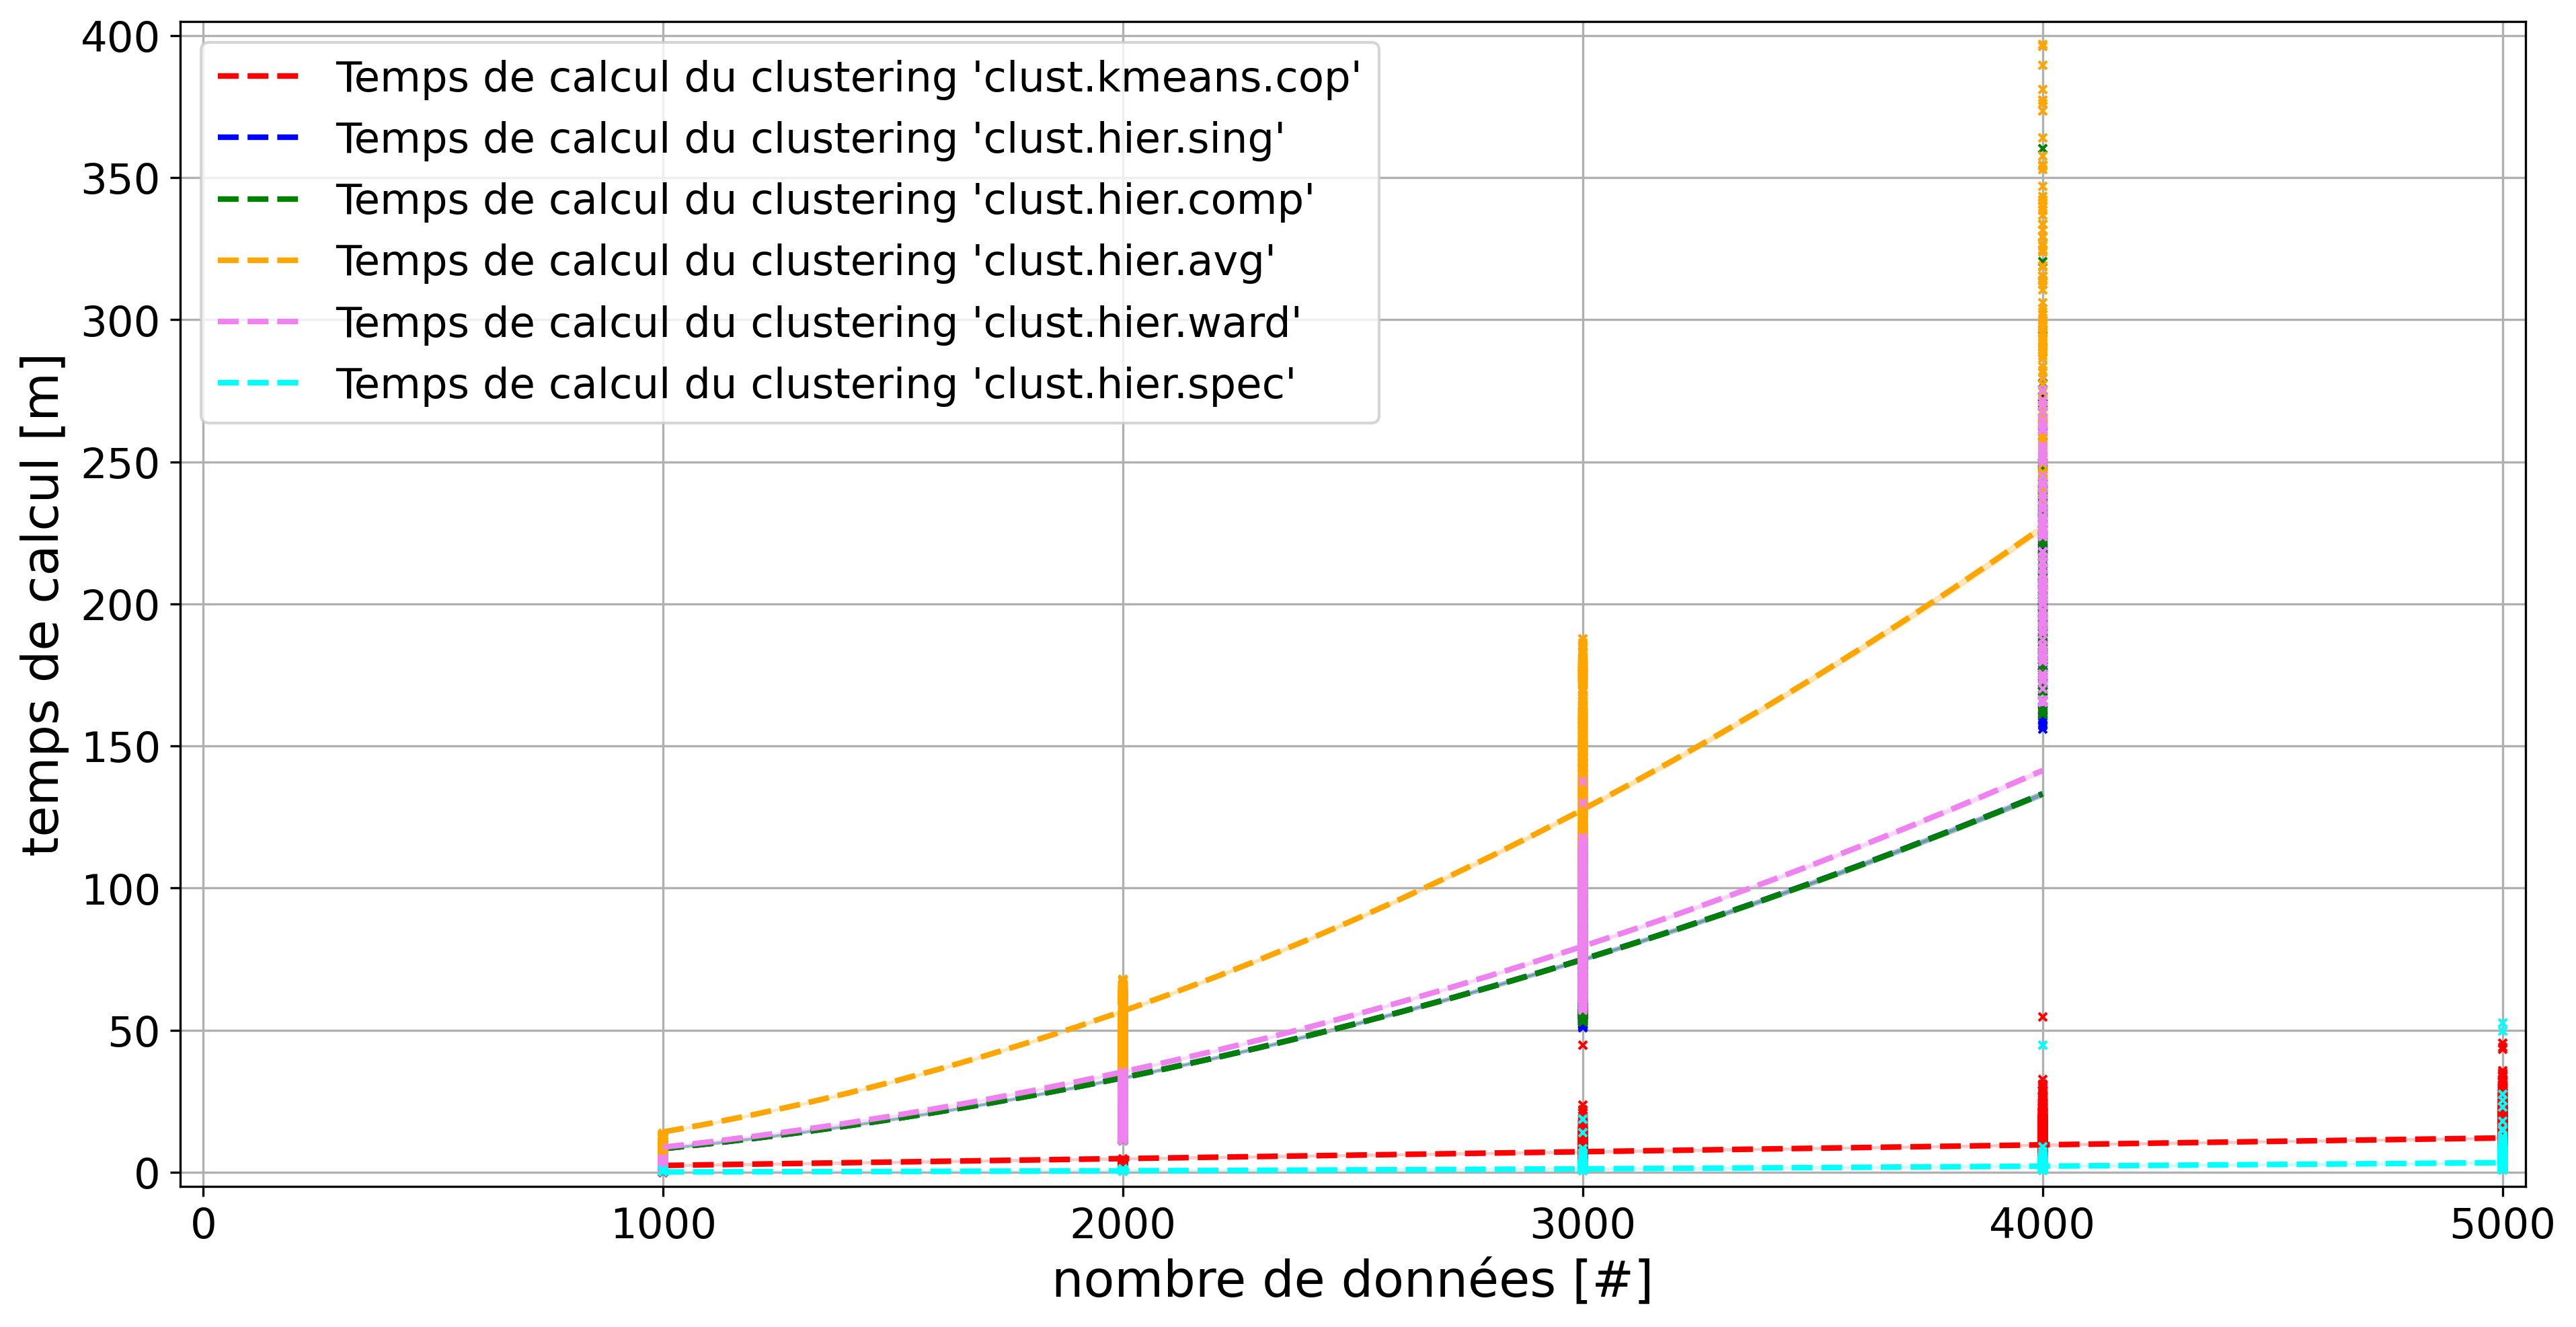
\includegraphics[width=0.8\textwidth]{figures/etude-temps-calcul-modelisation-3clust}
				\caption{Estimation du temps nécessaire (en secondes) pour effectuer une tâche de \textbf{clustering} en fonction du nombre de données à traiter.}
				\label{figure:4.3.2-ETUDE-COUTS-TEMPS-CALCUL-MODELISATION-CLUSTERING}
			\end{figure}
			
			%%% Sampling
			
			% Première analyse.
			En ce qui concerne la tâche d'\textbf{échantillonnage de contraintes}, une première analyse montre que les modélisations des quatre implémentations sont différentiables  (\texttt{p-valeur}: $<$ \texttt{$10^{-3}$}). Nous ferons donc une modélisation par algorithme.
			
			% Modélisation du temps de calcul (samp.rand.full).
			Pour les algorithmes de l'échantillonnage de contraintes \texttt{samp.rand.full}, l'analyse de la corrélation des facteurs avec les mesures de temps d'exécution indique qu'une modélisation minimale et suffisante peut être réalisée à partir du facteur $\texttt{dataset\_size}^{2}$ (\texttt{r}: $0.993$).
			Le second facteur le plus corrélé (mais non retenu) est l'interaction $\texttt{dataset\_size}^{2} \cdot previous\_nb\_clusters$ (\texttt{r}: $0.791$).
			Le modèle linéaire généralisé retenu (\texttt{R²}: $> 0.999$, \texttt{llf}: $-4.33 \cdot 10^{4}$, \texttt{llf\_null}: $-1.17 \cdot 10^{5}$) nous permet de déduire l'équation suivante\todo{ref annexe} :
			%
			\begin{equation}
				time(samp.rand.full)
				\simeq -4.78 \cdot 10^{-1} + 8.47 \cdot 10^{-7} \cdot \texttt{dataset\_size}^{2}
			\end{equation}
			
			% Modélisation du temps de calcul (samp.rand.same).
			Pour les algorithmes de l'échantillonnage de contraintes \texttt{samp.rand.same}, l'analyse de la corrélation des facteurs avec les mesures de temps d'exécution indique qu'une modélisation minimale et suffisante peut être réalisée à partir du facteur $\texttt{dataset\_size}^{2}$ (\texttt{r}: $0.939$).
			Le second facteur le plus corrélé (mais non retenu) est l'interaction $\texttt{dataset\_size}^{2} \cdot algorithm\_nb\_constraints$ (\texttt{r}: $0.611$).
			Le modèle linéaire généralisé retenu (\texttt{R²}: $> 0.999$, \texttt{llf}: $-3.17 \cdot 10^{4}$, \texttt{llf\_null}: $-6.84 \cdot 10^{4}$) nous permet de déduire l'équation suivante\todo{ref annexe} :
			%
			\begin{equation}
				time(samp.rand.same)
				\simeq -1.36 \cdot 10^{-1} + 1.92 \cdot 10^{-7} \cdot \texttt{dataset\_size}^{2}
			\end{equation}
			
			% Modélisation du temps de calcul (samp.farhtest.same).
			Pour les algorithmes de l'échantillonnage de contraintes \texttt{samp.farhtest.same}, l'analyse de la corrélation des facteurs avec les mesures de temps d'exécution indique qu'une modélisation minimale et suffisante peut être réalisée à partir du facteur $\texttt{dataset\_size}^{2}$ (\texttt{r}: $0.981$).
			Le second facteur le plus corrélé (mais non retenu) est l'interaction $\texttt{dataset\_size}^{2} \cdot previous\_nb\_clusters$ (\texttt{r}: $0.700$).
			Le modèle linéaire généralisé retenu (\texttt{R²}: $> 0.999$, \texttt{llf}: $-4.52 \cdot 10^{4}$, \texttt{llf\_null}: $-1.02 \cdot 10^{5}$) nous permet de déduire l'équation suivante\todo{ref annexe} :
			%
			\begin{equation}
				time(samp.farhtest.same)
				\simeq -2.25 \cdot 10^{-1} + 5.32 \cdot 10^{-7} \cdot \texttt{dataset\_size}^{2}
			\end{equation}
			
			% Modélisation du temps de calcul (samp.closest.diff).
			Pour les algorithmes de l'échantillonnage de contraintes \texttt{samp.closest.diff}, l'analyse de la corrélation des facteurs avec les mesures de temps d'exécution indique qu'une modélisation minimale et suffisante peut être réalisée à partir du facteur $\texttt{dataset\_size}^{2}$ (\texttt{r}: $0.995$).
			Le second facteur le plus corrélé (mais non retenu) est l'interaction $\texttt{dataset\_size}^{2} \cdot previous\_nb\_clusters$ (\texttt{r}: $0.815$).
			Le modèle linéaire généralisé retenu (\texttt{R²}: $> 0.999$, \texttt{llf}: $-5.80 \cdot 10^{4}$, \texttt{llf\_null}: $-1.36 \cdot 10^{5}$) nous permet de déduire l'équation suivante\todo{ref annexe} :
			%
			\begin{equation}
				time(samp.closest.diff)
				\simeq -6.58 \cdot 10^{-1} + 1.46 \cdot 10^{-6} \cdot \texttt{dataset\_size}^{2}
			\end{equation}
			
			% Affichage du temps de calcul.
			La figure~\ref{figure:4.3.2-ETUDE-COUTS-TEMPS-CALCUL-MODELISATION-SAMPLING} représente ces modélisations de temps de calcul des algorithmes d'échantillonnage en comparaison avec les mesures réalisées lors de l'expérience.
			\newline
			%
			\begin{figure}[!htb]
				\centering
				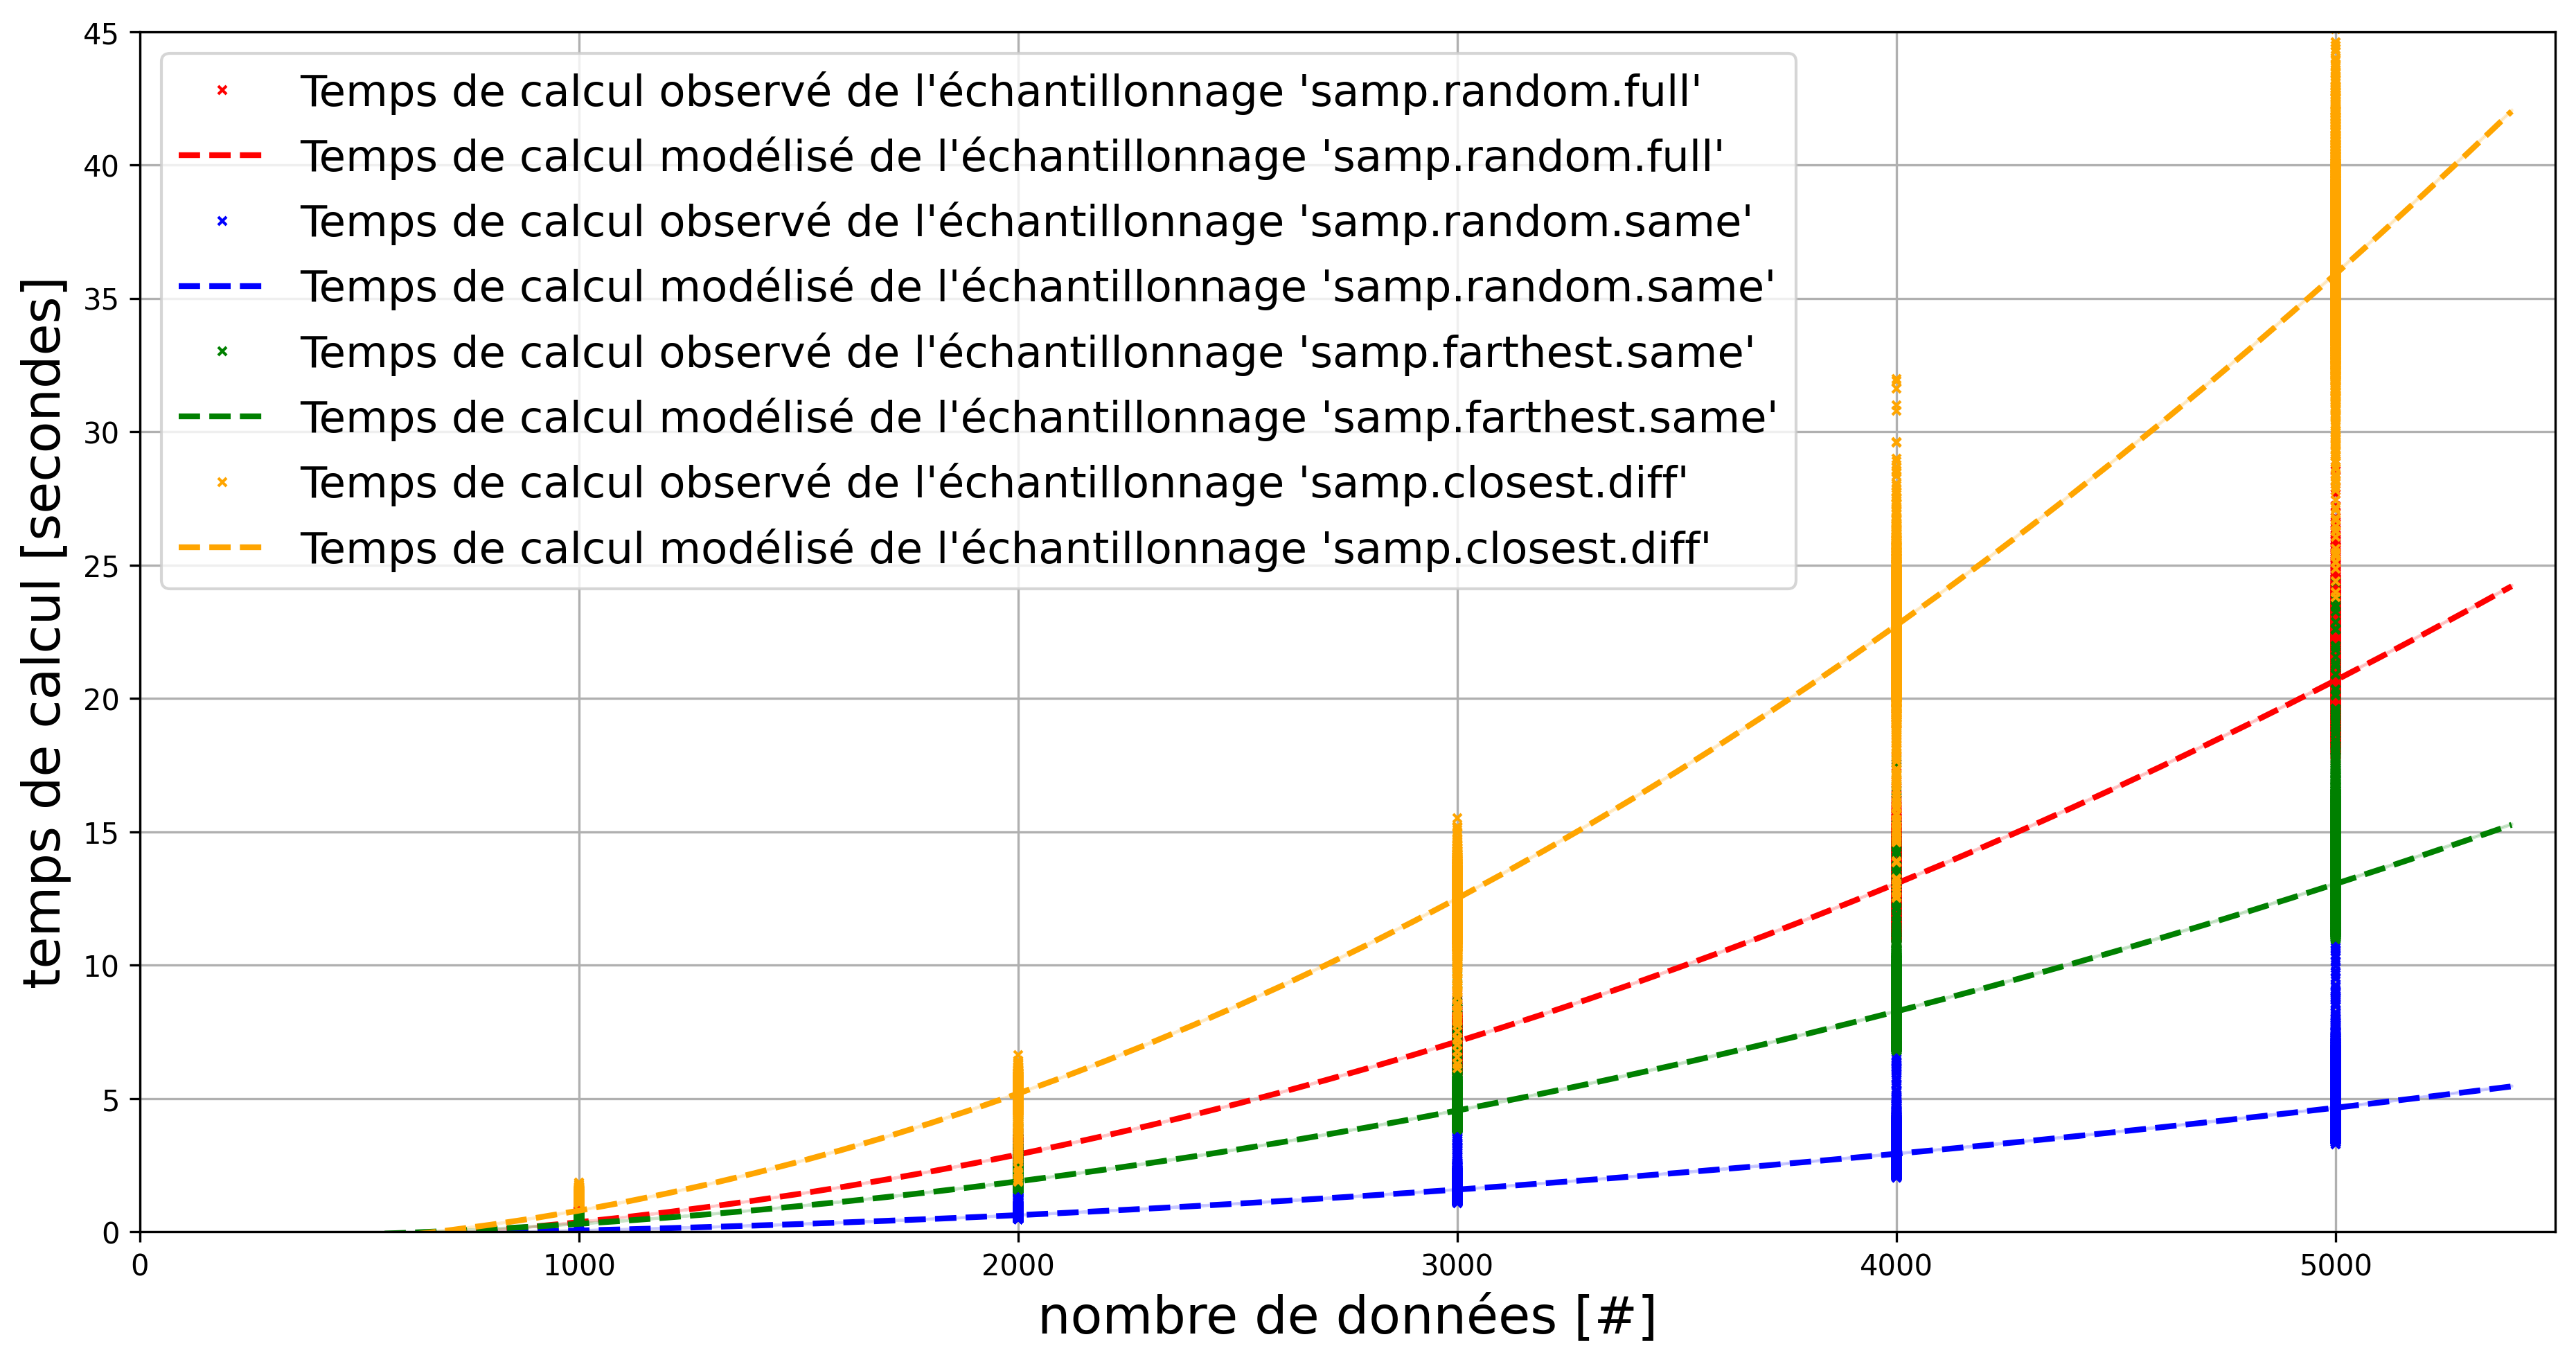
\includegraphics[width=0.8\textwidth]{figures/etude-temps-calcul-modelisation-4samp}
				\caption{Estimation du temps nécessaire (en secondes) pour effectuer une tâche d'\textbf{échantillonnage de contraintes} en fonction du nombre de données à traiter.}
				\label{figure:4.3.2-ETUDE-COUTS-TEMPS-CALCUL-MODELISATION-SAMPLING}
			\end{figure}

		%%% Discussion
		\subsubsection{Discussion}
		
			% Rappel de l'objectif : estimer le temps d'exécution.
			Dans cette étude, nous avons estimé le temps de calcul des différents algorithmes implémentés afin de confirmer le choix de paramétrage pour une convergence optimal (cf. hypothèse d'efficience en section~\ref{section:4.2-HYPOTHESE-EFFICIENCE}).
			Ces estimations ont été réalisées sur la base de plusieurs exécutions et fonction de divers contextes d'utilisation : nombre de données, nombre de contraintes annotées, nombre de contraintes à sélectionner, nombre de \textit{clusters} existant, nombre de \textit{clusters} à trouver.
			
			% Remarque générale : Dépend principalement du nombre de données.
			En premier lieu, on peut constater que les différentes modélisations dépendent majoritairement de la taille du jeu de données manipulé ($\texttt{dataset\_size}$ ou $\texttt{dataset\_size}^{2}$) avec un score de corrélation \texttt{r} avec le temps mesuré généralement supérieur à $0.9$ et des modèles \textit{GLM} avec des coefficients de détermination généralisé \texttt{R²} généralement proches de $0.999$.
			Bien que d'autres facteurs peuvent intervenir dans ces estimations (notamment les interactions doubles entre la taille du jeu de données et le nombre de \textit{clusters} ou le nombre de contraintes), ces derniers semblent avoir un impact négligeable sur le temps d'exécution.
			
			% Note: remarque sur le nombre de contraintes.
			\begin{leftBarAuthorOpinion}
				Certains paramétrages de la méthode du \textit{clustering} interactif semblent cependant avoir un temps de calcul décroissant au cours des itérations, mais nous n'avons cependant pas pu montrer de tendances globales significatives.
				Il est probable que l'ajout de contraintes judicieusement placées permettent à certains algorithmes de \textit{clustering} de s'exécuter plus rapidement, notamment lorsque ceux-ci exploitent les composants connexes du graphe de contraintes (cf. section~\ref{section:3.3.2-GESTION-DES-CONTRAINTES}). En effet, :
				\begin{itemize}
					\item les \textit{clustering} hiérarchiques s'initialisent autant de \textit{clusters} que de groupes de données liées entre elles par des contraintes \texttt{MUST-LINK} : or s'il y a plus de contraintes, alors les composants connexes sont davantage développés, donc il y a moins de \textit{clusters} à initialiser et donc moins d'époques de l'algorithme ;
					\item le \textit{clustering} KMeans (modèle COP) attire auprès d'un barycentre l'ensemble des données liées par un \texttt{MUST-LINK} : or s'il y a plus de contraintes, alors il y a des données attirées, donc les noyaux de \textit{clusters} peuvent se stabiliser plus rapidement.  
				\end{itemize}
				Toutefois, ces suppositions n'ont pas pu être démontrées, et certains contre-exemples tendent à conclure que ces comportements sont très dépendants du jeu de données manipulé et de l'ordre d'ajout des contraintes. Par exemple :
				\begin{itemize}
					\item l'ajout d'un trop grand nombre de contraintes \texttt{CANNOT-LINK} peut engendrer un surplus de vérification pour estimer quelles formations de \textit{clusters} sont autorisées sans violer de contraintes ;
					\item l'algorithme KMeans (modèle COP) peut osciller autour de plusieurs noyaux de \textit{clusters} instables si les contraintes violent trop la similarité intrinsèque des données.
				\end{itemize}
			\end{leftBarAuthorOpinion}
			
			% Cas du clustering.
			En ce qui concerne la tâche de \textit{clustering}, on note des différences significatives dans les temps d'exécution des divers algorithmes implémentés.
			En effet, l'algorithme KMeans (modèle COP) est nettement plus rapide (complexité en $ \mathcal{O}(\texttt{dataset\_size}) $, nécessitant quelques dizaines de minutes pour $5~000$ données) que les implémentations du \textit{clustering} hiérarchique (complexité en $ \mathcal{O}(\texttt{dataset\_size}^{2}) $, nécessitant plusieurs heures pour $5~000$ données).
			Cette différence, visible en figure~\ref{figure:4.3.2-ETUDE-COUTS-TEMPS-CALCUL-MODELISATION-CLUSTERING}, a un réel impact sur l'expérience utilisateur de l'opérateur.
			En effet, bien qu'il soit théoriquement plus efficient pour atteindre une annotation suffisante (cf. hypothèse d'efficience en section~\ref{section:4.2-HYPOTHESE-EFFICIENCE}), l'usage d'un \textit{clustering} hiérarchique imposerait de longs temps d'attente à l'opérateur, interdisant des interactions rapides avec la machines.
			Or l'intérêt principal de notre méthodologie d'annotation à l'aide du \textit{clustering} interactif repose sur ces interactions homme-machine via l'ajout régulier de contraintes pertinentes (cf. hypothèse d'efficacité en section~\ref{section:4.1-HYPOTHESE-EFFICACITE}).
			Nous décidons donc d'exclure l'usage des algorithmes de \textit{clustering} hiérarchique au profit du \textit{clustering} KMeans (modèle COP).
			
			% Note: Cas du projet étudiant avec TPS.
			\begin{leftBarInformation}
				Dans le cadre du projet étudiant avec l'école Télécom Physique Strasbourg visant à implémenter d'autres algorithmes de \textit{clustering} sous contraintes, un résonnement similaire a été utilisé pour filtrer les algorithmes. Ainsi, l'implémentation de KMeans (modèle MPC) a été exclu (complexité en $ \mathcal{O}(\texttt{dataset\_size}^{3}) $) et l'implémentation de la propagation par affinité écarte la gestion des contraintes \texttt{CANNOT-LINK} pour avoir un temps d'exécution comparable au \textit{clustering} KMeans (modèle COP). L'algorithme DBScan (modèle C-DBScan) est quand à lui un rival possible avec une complexité théorique en $ \mathcal{O}(\texttt{dataset\_size}) $.
			\end{leftBarInformation}
			% Note: Cas du KMeans.
			
			% Cas du prétraitement + vectorisation + échantillonage.
			En ce qui concerne les tâches de prétraitements (figure~\ref{figure:4.3.2-ETUDE-COUTS-TEMPS-CALCUL-MODELISATION-PREPROCESSING}), de vectorisation (figure~\ref{figure:4.3.2-ETUDE-COUTS-TEMPS-CALCUL-MODELISATION-VECTORIZATION}), et d'échantillonnage de contraintes (cf. figure~\ref{figure:4.3.2-ETUDE-COUTS-TEMPS-CALCUL-MODELISATION-SAMPLING}) ont des complexités presque négligeables au regard des temps d'exécution du \textit{clustering} (pour $5~000$ données : environ $60$ secondes contre près de $800$ secondes pour \texttt{clust.kmeans.cop} et près de $15~000$ secondes pour \texttt{clust.hier.sing}).
			Nous maintenons donc les paramétrages obtenus pour ces tâches en section~\ref{section:4.2-HYPOTHESE-EFFICIENCE} sans analyses complémentaires et bornons l'ensemble des ces temps de calcul par un temps constant de $60$ secondes.
			
			% Conclusion.
			Pour conclure, dans l'optique d'atteindre de manière efficiente $90$\% de v-measure (annotation partielle) avec un coût global minimal, nous retenons l'usage du \textbf{paramétrage favori} constitué du prétraitement simple (\texttt{prep.simple}), de la vectorisation TF-IDF (\texttt{vect.tfidf}), du clustering KMeans avec modèle COP (\texttt{clust.kmeans.cop}) et de l'échantillonnage des données les plus proches dans des clusters différents (\texttt{sampl.closest.diff}).
			On estime le temps d'exécution de ce paramétrage avec l'équation suivante\footnote{Pour $1~000$ données : environ $30$ secondes ; Pour $5~000$ données : environ $15$ minutes.} :
			%
			\begin{equation}
				time(parametrage.favori)
				\simeq -1.80 \cdot 10^{2} + 2.11 \cdot 10^{-1} \cdot \texttt{dataset\_size}
			\end{equation}
			
			% Ouverture sur le temps de coût total.
			Pour poursuivre cette étude et estimer le coût total de la méthode, nous devons maintenant estimer le nombre moyen d'itérations nécessaires de la méthode en fonction de la taille du jeu de données à annoter (cf. section~\ref{section:4.3.3-ETUDE-COUT-NOMBRE-CONTRAINTES}).
	
	%%%
	%%% Subsection 4.3.3: Étude du nombre de contraintes nécessaires
	%%%
	\subsection{Étude du nombre de contraintes nécessaires}
	\label{section:4.3.3-ETUDE-COUT-NOMBRE-CONTRAINTES}
	
		%%% Protocole expérimental.
		\subsubsection{Protocole expérimental}

			% Objectif de l'expérience.
			\todo[inline]{A REDIGER:}
			% Détails de l'expérience.
			\todo[inline]{A REDIGER:}
			% Description des tâches, des algorithmes et des paramètres.
			\todo[inline]{A REDIGER:}
			% Description de l'évaluation.
			\todo[inline]{A REDIGER:}
			% Pseudo-code.
			\todo[inline]{A REDIGER:}

			% Référence scripts.
			\begin{leftBarInformation}
				Les scripts de l'expérience (\textit{notebooks} Python) sont disponibles dans un dossier dédié de~\cite{schild:cognitivefactory-interactive-clustering-comparative-study:2021}.
			\end{leftBarInformation}

		%%% Résultats
		\subsubsection{Résultats obtenus}

		%%% Discussion
		\subsubsection{Discussion}
	
	%%%
	%%% Subsection 4.3.4: Estimation du temps total d'un projet d'annotation
	%%%
	\subsection{Estimation du temps total d'un projet d'annotation}
	\label{section:4.3.4-ETUDE-COUTS-TOTAL}
	
		%%% Protocole expérimental.
		\subsubsection{Protocole expérimental}
		
			% Objectif de l'expérience.
			\todo[inline]{A REDIGER:}
			% Détails de l'expérience.
			\todo[inline]{A REDIGER:}
			% Description des tâches, des algorithmes et des paramètres.
			\todo[inline]{A REDIGER:}
			% Description de l'évaluation.
			\todo[inline]{A REDIGER:}
			% Pseudo-code.
			\todo[inline]{A REDIGER:}

			% Référence scripts.
			\begin{leftBarInformation}
				Les scripts de l'expérience (\textit{notebooks} Python) sont disponibles dans un dossier dédié de~\cite{schild:cognitivefactory-interactive-clustering-comparative-study:2021}.
			\end{leftBarInformation}

		%%% Résultats
		\subsubsection{Résultats obtenus}

		%%% Discussion
		\subsubsection{Discussion}